% Options for packages loaded elsewhere
\PassOptionsToPackage{unicode}{hyperref}
\PassOptionsToPackage{hyphens}{url}
%
\documentclass[
]{article}
\usepackage{amsmath,amssymb}
\usepackage{iftex}
\ifPDFTeX
  \usepackage[T1]{fontenc}
  \usepackage[utf8]{inputenc}
  \usepackage{textcomp} % provide euro and other symbols
\else % if luatex or xetex
  \usepackage{unicode-math} % this also loads fontspec
  \defaultfontfeatures{Scale=MatchLowercase}
  \defaultfontfeatures[\rmfamily]{Ligatures=TeX,Scale=1}
\fi
\usepackage{lmodern}
\ifPDFTeX\else
  % xetex/luatex font selection
\fi
% Use upquote if available, for straight quotes in verbatim environments
\IfFileExists{upquote.sty}{\usepackage{upquote}}{}
\IfFileExists{microtype.sty}{% use microtype if available
  \usepackage[]{microtype}
  \UseMicrotypeSet[protrusion]{basicmath} % disable protrusion for tt fonts
}{}
\makeatletter
\@ifundefined{KOMAClassName}{% if non-KOMA class
  \IfFileExists{parskip.sty}{%
    \usepackage{parskip}
  }{% else
    \setlength{\parindent}{0pt}
    \setlength{\parskip}{6pt plus 2pt minus 1pt}}
}{% if KOMA class
  \KOMAoptions{parskip=half}}
\makeatother
\usepackage{xcolor}
\usepackage[margin=1in]{geometry}
\usepackage{color}
\usepackage{fancyvrb}
\newcommand{\VerbBar}{|}
\newcommand{\VERB}{\Verb[commandchars=\\\{\}]}
\DefineVerbatimEnvironment{Highlighting}{Verbatim}{commandchars=\\\{\}}
% Add ',fontsize=\small' for more characters per line
\usepackage{framed}
\definecolor{shadecolor}{RGB}{248,248,248}
\newenvironment{Shaded}{\begin{snugshade}}{\end{snugshade}}
\newcommand{\AlertTok}[1]{\textcolor[rgb]{0.94,0.16,0.16}{#1}}
\newcommand{\AnnotationTok}[1]{\textcolor[rgb]{0.56,0.35,0.01}{\textbf{\textit{#1}}}}
\newcommand{\AttributeTok}[1]{\textcolor[rgb]{0.13,0.29,0.53}{#1}}
\newcommand{\BaseNTok}[1]{\textcolor[rgb]{0.00,0.00,0.81}{#1}}
\newcommand{\BuiltInTok}[1]{#1}
\newcommand{\CharTok}[1]{\textcolor[rgb]{0.31,0.60,0.02}{#1}}
\newcommand{\CommentTok}[1]{\textcolor[rgb]{0.56,0.35,0.01}{\textit{#1}}}
\newcommand{\CommentVarTok}[1]{\textcolor[rgb]{0.56,0.35,0.01}{\textbf{\textit{#1}}}}
\newcommand{\ConstantTok}[1]{\textcolor[rgb]{0.56,0.35,0.01}{#1}}
\newcommand{\ControlFlowTok}[1]{\textcolor[rgb]{0.13,0.29,0.53}{\textbf{#1}}}
\newcommand{\DataTypeTok}[1]{\textcolor[rgb]{0.13,0.29,0.53}{#1}}
\newcommand{\DecValTok}[1]{\textcolor[rgb]{0.00,0.00,0.81}{#1}}
\newcommand{\DocumentationTok}[1]{\textcolor[rgb]{0.56,0.35,0.01}{\textbf{\textit{#1}}}}
\newcommand{\ErrorTok}[1]{\textcolor[rgb]{0.64,0.00,0.00}{\textbf{#1}}}
\newcommand{\ExtensionTok}[1]{#1}
\newcommand{\FloatTok}[1]{\textcolor[rgb]{0.00,0.00,0.81}{#1}}
\newcommand{\FunctionTok}[1]{\textcolor[rgb]{0.13,0.29,0.53}{\textbf{#1}}}
\newcommand{\ImportTok}[1]{#1}
\newcommand{\InformationTok}[1]{\textcolor[rgb]{0.56,0.35,0.01}{\textbf{\textit{#1}}}}
\newcommand{\KeywordTok}[1]{\textcolor[rgb]{0.13,0.29,0.53}{\textbf{#1}}}
\newcommand{\NormalTok}[1]{#1}
\newcommand{\OperatorTok}[1]{\textcolor[rgb]{0.81,0.36,0.00}{\textbf{#1}}}
\newcommand{\OtherTok}[1]{\textcolor[rgb]{0.56,0.35,0.01}{#1}}
\newcommand{\PreprocessorTok}[1]{\textcolor[rgb]{0.56,0.35,0.01}{\textit{#1}}}
\newcommand{\RegionMarkerTok}[1]{#1}
\newcommand{\SpecialCharTok}[1]{\textcolor[rgb]{0.81,0.36,0.00}{\textbf{#1}}}
\newcommand{\SpecialStringTok}[1]{\textcolor[rgb]{0.31,0.60,0.02}{#1}}
\newcommand{\StringTok}[1]{\textcolor[rgb]{0.31,0.60,0.02}{#1}}
\newcommand{\VariableTok}[1]{\textcolor[rgb]{0.00,0.00,0.00}{#1}}
\newcommand{\VerbatimStringTok}[1]{\textcolor[rgb]{0.31,0.60,0.02}{#1}}
\newcommand{\WarningTok}[1]{\textcolor[rgb]{0.56,0.35,0.01}{\textbf{\textit{#1}}}}
\usepackage{graphicx}
\makeatletter
\def\maxwidth{\ifdim\Gin@nat@width>\linewidth\linewidth\else\Gin@nat@width\fi}
\def\maxheight{\ifdim\Gin@nat@height>\textheight\textheight\else\Gin@nat@height\fi}
\makeatother
% Scale images if necessary, so that they will not overflow the page
% margins by default, and it is still possible to overwrite the defaults
% using explicit options in \includegraphics[width, height, ...]{}
\setkeys{Gin}{width=\maxwidth,height=\maxheight,keepaspectratio}
% Set default figure placement to htbp
\makeatletter
\def\fps@figure{htbp}
\makeatother
\usepackage{svg}
\setlength{\emergencystretch}{3em} % prevent overfull lines
\providecommand{\tightlist}{%
  \setlength{\itemsep}{0pt}\setlength{\parskip}{0pt}}
\setcounter{secnumdepth}{-\maxdimen} % remove section numbering
\ifLuaTeX
  \usepackage{selnolig}  % disable illegal ligatures
\fi
\IfFileExists{bookmark.sty}{\usepackage{bookmark}}{\usepackage{hyperref}}
\IfFileExists{xurl.sty}{\usepackage{xurl}}{} % add URL line breaks if available
\urlstyle{same}
\hypersetup{
  pdftitle={Tidyverse},
  pdfauthor={Teresa Vaz Martins},
  hidelinks,
  pdfcreator={LaTeX via pandoc}}

\title{Tidyverse}
\author{Teresa Vaz Martins}
\date{2024-01-08}

\begin{document}
\maketitle

\#This is the tidyverse session for the R course 2025. It was based on
the original \#tidyverse session by Teresa Vas Martins (2024) but Kate
Dewally has made a few \#minor edits

\begin{center}\rule{0.5\linewidth}{0.5pt}\end{center}

\textbf{Learning objectives:}

In this session:

\begin{itemize}
\item
  what is the tidyverse and why you should use it
\item
  install the tidyverse
\item
  very brief overview of core functionality and a few available tools
\end{itemize}

In the following sessions, you will have the opportunity to use the
tidyverse in practice

\begin{center}\rule{0.5\linewidth}{0.5pt}\end{center}

\hypertarget{the-data-science-life-cycle}{%
\section{The Data Science Life
Cycle}\label{the-data-science-life-cycle}}

Scientists use data to answer a question, with a number of steps
in-between: need to identify relevant data, import it, transform into a
format that is easy to work with, explore, possibly visualise, analyse,
and communicate their findings.

A typical data science life cycle consists of the following stages:

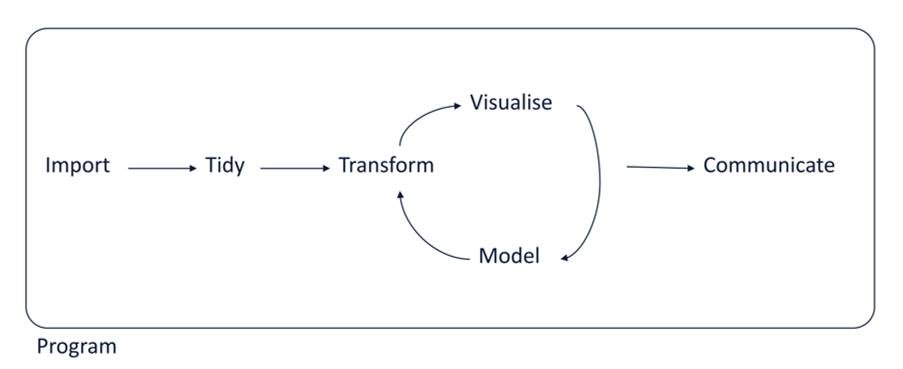
\includegraphics{data_pipeline.png}

Source: \href{https://r4ds.hadley.nz/}{R for Data Science (2e)
(hadley.nz)}, Hadley Wickham.

\begin{center}\rule{0.5\linewidth}{0.5pt}\end{center}

\hypertarget{what-is-the-tidyverse}{%
\section{What is the tidyverse}\label{what-is-the-tidyverse}}

The tidyverse is ``an opinionated collection of R packages designed for
data science. All packages share an underlying design philosophy,
grammar, and data structures.'' Specifically, it is:

\begin{center}\rule{0.5\linewidth}{0.5pt}\end{center}

\begin{itemize}
\tightlist
\item
  \textbf{a metadata package: i}f you install the tidyverse
  (\texttt{install.packages(\textquotesingle{}tidyverse\textquotesingle{}}),
  you will automatically install a set of core packages that provide
  consistent solutions to various steps of the data life cycle
\end{itemize}

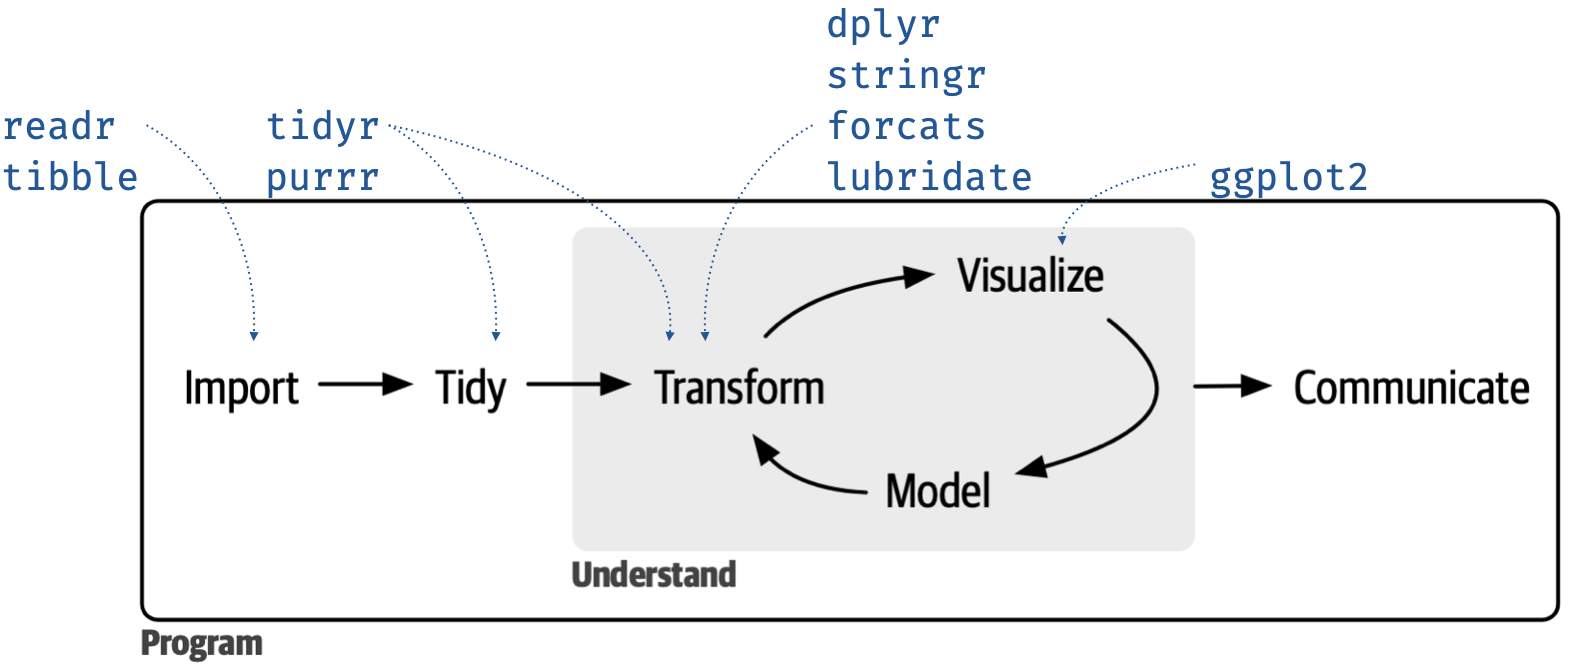
\includegraphics{data-science.png}

Source:
\url{https://www.tidyverse.org/blog/2023/08/teach-tidyverse-23/\#improved-and-expanded-_join-functionality}

\begin{center}\rule{0.5\linewidth}{0.5pt}\end{center}

\begin{itemize}
\tightlist
\item
  \textbf{a R dialect:} alongside the core packages, there is a growing
  number of tidyverse-adjacent packages built on the same principles,
  designed to integrate consistently with the tidyverse. The below is
  just a small sample (some are official but non-core tidyverse, like
  and others, like for instance Shiny and rmarkdown are not yet part of
  the official tidyverse)
\end{itemize}

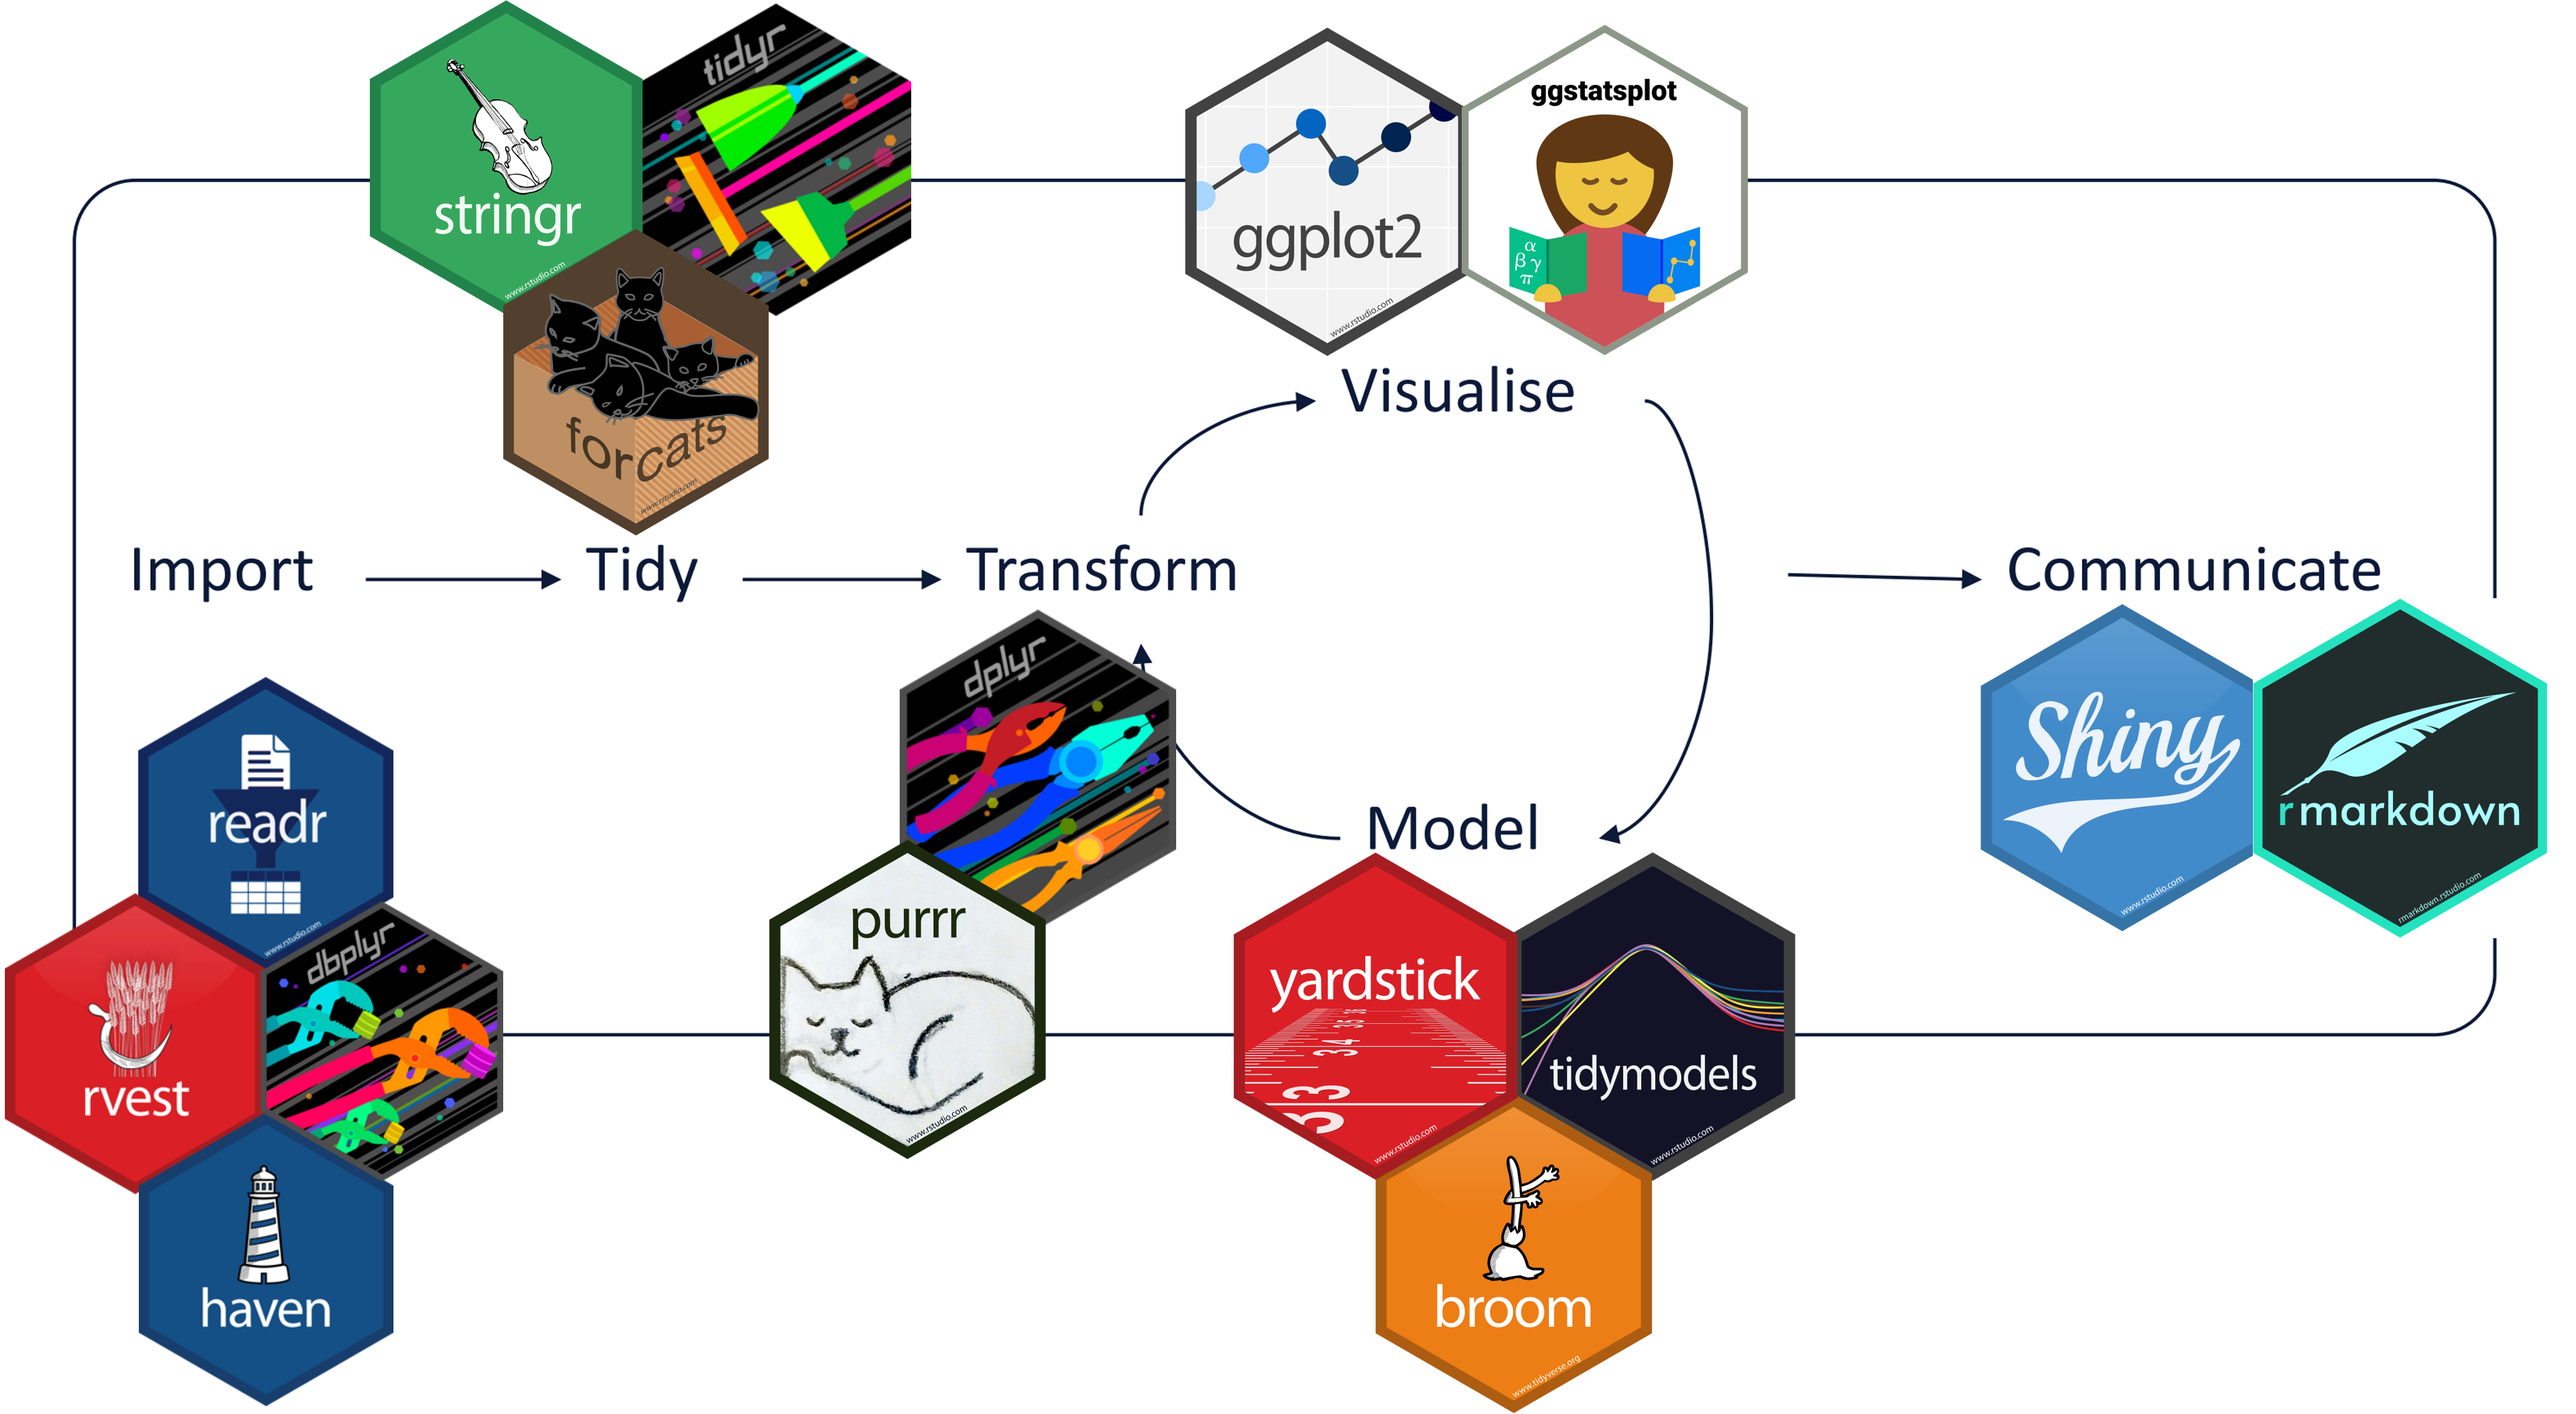
\includegraphics{tidypipe.png}

\begin{center}\rule{0.5\linewidth}{0.5pt}\end{center}

\begin{itemize}
\tightlist
\item
  \textbf{maybe a R subcommunity?} There is a very large number of
  guidelines and resources to promote, teach and provide support for
  this ``\textbf{opinionated} collection of R packages''. For instance,
  see:
\end{itemize}

\textbf{understand the principles} (including code of conduct!)

\url{https://design.tidyverse.org/unifying.html}
(\emph{``\textbf{inclusive}, because the tidyverse is not just the
collection of packages, but it is also the community of people who use
them.'')}

\begin{center}\rule{0.5\linewidth}{0.5pt}\end{center}

\hypertarget{what-the-tidyverse-is-not}{%
\subsection{What the tidyverse is not}\label{what-the-tidyverse-is-not}}

\begin{itemize}
\item
  \textbf{not a replacement of base R} (base R is the default R
  installation).

  \begin{itemize}
  \tightlist
  \item
    the tidyverse is built on top of base R, not meant to replace it
  \end{itemize}
\item
  \textbf{not something that demands exclusivity}

  \begin{itemize}
  \tightlist
  \item
    There are other useful dialects (the faster \texttt{data.table}, for
    instance) and you don't need to stick with one exclusively. A
    typical script may combine different dialects
  \end{itemize}
\item
  \textbf{not something that you need to keep up with anxiously}

  \begin{itemize}
  \item
    the tidyverse has a very fast update rate.
  \item
    during the time scale of a research project of about 2 or 3 years,
    you may find that the tidyverse syntax has changed. It doesn't mean
    that your code has become obsolete. If you have doubts about a
    particular function, you can consult its state (write ?gather in the
    console)): by default, functions are in a stable state, but:

    \url{https://lifecycle.r-lib.org/articles/stages.html\#superseded}

    \emph{Superseded functions will not receive new features, but will
    receive any critical bug fixes needed to keep it working. In some
    ways a superseded function is actually safer than a stable function
    because it\textquotesingle s guaranteed never to change (for better
    or for worse).}
  \end{itemize}
\end{itemize}

\includesvg{lifecycle.svg}

\begin{center}\rule{0.5\linewidth}{0.5pt}\end{center}

\hypertarget{how-to-install-the-tidyverse}{%
\section{How to install the
tidyverse}\label{how-to-install-the-tidyverse}}

\begin{Shaded}
\begin{Highlighting}[]
\CommentTok{\# Package names}
\NormalTok{packages }\OtherTok{\textless{}{-}} \FunctionTok{c}\NormalTok{(}\StringTok{\textquotesingle{}tidyverse\textquotesingle{}}\NormalTok{, }\StringTok{\textquotesingle{}palmerpenguins\textquotesingle{}}\NormalTok{, }\StringTok{\textquotesingle{}ViewPipeSteps\textquotesingle{}}\NormalTok{)}
              
\CommentTok{\# Install packages not yet installed}
\NormalTok{installed\_packages }\OtherTok{\textless{}{-}}\NormalTok{ packages }\SpecialCharTok{\%in\%} \FunctionTok{rownames}\NormalTok{(}\FunctionTok{installed.packages}\NormalTok{())}
\ControlFlowTok{if}\NormalTok{ (}\FunctionTok{any}\NormalTok{(installed\_packages }\SpecialCharTok{==} \ConstantTok{FALSE}\NormalTok{)) \{}
  \FunctionTok{install.packages}\NormalTok{(packages[}\SpecialCharTok{!}\NormalTok{installed\_packages], }\AttributeTok{repos =} \StringTok{"http://cran.us.r{-}project.org"}\NormalTok{)}
\NormalTok{\}}

\CommentTok{\# Packages loading}
\FunctionTok{invisible}\NormalTok{(}\FunctionTok{lapply}\NormalTok{(packages, library, }\AttributeTok{character.only =} \ConstantTok{TRUE}\NormalTok{))}
\end{Highlighting}
\end{Shaded}

\begin{itemize}
\tightlist
\item
  you can also install each package separately using the command
  install.packages(``NAME OF PACKAGE'')
\end{itemize}

\begin{center}\rule{0.5\linewidth}{0.5pt}\end{center}

\hypertarget{two-essential-tools-pipes-and-tidy-data}{%
\section{Two essential tools: pipes and tidy
data}\label{two-essential-tools-pipes-and-tidy-data}}

\begin{center}\rule{0.5\linewidth}{0.5pt}\end{center}

\hypertarget{pipes}{%
\subsection{Pipes}\label{pipes}}

The maigrittr \texttt{magrittr::\%\textgreater{}\%} allows us to chain
several chunks of code together

\textbf{Avoid using the pipe when:}

\begin{itemize}
\item
  You need to manipulate more than one object at a time. Reserve pipes
  for a sequence of steps applied to one primary object.
\item
  There are meaningful intermediate objects that could be given
  informative names.

  \begin{center}\rule{0.5\linewidth}{0.5pt}\end{center}
\end{itemize}

\hypertarget{why-use-the-pipe-in-other-cases}{%
\subsubsection{Why use the pipe in other
cases?}\label{why-use-the-pipe-in-other-cases}}

Piping is used to emphasise a sequence of actions and avoid nested
operations. Let's see the alternatives:

\hypertarget{multiple-lines-of-code}{%
\paragraph{Multiple lines of code}\label{multiple-lines-of-code}}

\begin{Shaded}
\begin{Highlighting}[]
\NormalTok{penguins }\OtherTok{\textless{}{-}}\NormalTok{ palmerpenguins}\SpecialCharTok{::}\NormalTok{penguins }

\CommentTok{\# load data}
\NormalTok{data }\OtherTok{\textless{}{-}}\NormalTok{ palmerpenguins}\SpecialCharTok{::}\NormalTok{penguins\_raw }

\CommentTok{\#Visualise the data}
\FunctionTok{glimpse}\NormalTok{(data) }\CommentTok{\# switches rows and columns on display to allow you to see every column of data}
\end{Highlighting}
\end{Shaded}

\begin{verbatim}
## Rows: 344
## Columns: 17
## $ studyName             <chr> "PAL0708", "PAL0708", "PAL0708", "PAL0708", "PAL~
## $ `Sample Number`       <dbl> 1, 2, 3, 4, 5, 6, 7, 8, 9, 10, 11, 12, 13, 14, 1~
## $ Species               <chr> "Adelie Penguin (Pygoscelis adeliae)", "Adelie P~
## $ Region                <chr> "Anvers", "Anvers", "Anvers", "Anvers", "Anvers"~
## $ Island                <chr> "Torgersen", "Torgersen", "Torgersen", "Torgerse~
## $ Stage                 <chr> "Adult, 1 Egg Stage", "Adult, 1 Egg Stage", "Adu~
## $ `Individual ID`       <chr> "N1A1", "N1A2", "N2A1", "N2A2", "N3A1", "N3A2", ~
## $ `Clutch Completion`   <chr> "Yes", "Yes", "Yes", "Yes", "Yes", "Yes", "No", ~
## $ `Date Egg`            <date> 2007-11-11, 2007-11-11, 2007-11-16, 2007-11-16,~
## $ `Culmen Length (mm)`  <dbl> 39.1, 39.5, 40.3, NA, 36.7, 39.3, 38.9, 39.2, 34~
## $ `Culmen Depth (mm)`   <dbl> 18.7, 17.4, 18.0, NA, 19.3, 20.6, 17.8, 19.6, 18~
## $ `Flipper Length (mm)` <dbl> 181, 186, 195, NA, 193, 190, 181, 195, 193, 190,~
## $ `Body Mass (g)`       <dbl> 3750, 3800, 3250, NA, 3450, 3650, 3625, 4675, 34~
## $ Sex                   <chr> "MALE", "FEMALE", "FEMALE", NA, "FEMALE", "MALE"~
## $ `Delta 15 N (o/oo)`   <dbl> NA, 8.94956, 8.36821, NA, 8.76651, 8.66496, 9.18~
## $ `Delta 13 C (o/oo)`   <dbl> NA, -24.69454, -25.33302, NA, -25.32426, -25.298~
## $ Comments              <chr> "Not enough blood for isotopes.", NA, NA, "Adult~
\end{verbatim}

\begin{Shaded}
\begin{Highlighting}[]
\FunctionTok{head}\NormalTok{(data, }\DecValTok{5}\NormalTok{) }\CommentTok{\# gives you first few rows of dataframe (in this case 5)}
\end{Highlighting}
\end{Shaded}

\begin{verbatim}
## # A tibble: 5 x 17
##   studyName `Sample Number` Species          Region Island Stage `Individual ID`
##   <chr>               <dbl> <chr>            <chr>  <chr>  <chr> <chr>          
## 1 PAL0708                 1 Adelie Penguin ~ Anvers Torge~ Adul~ N1A1           
## 2 PAL0708                 2 Adelie Penguin ~ Anvers Torge~ Adul~ N1A2           
## 3 PAL0708                 3 Adelie Penguin ~ Anvers Torge~ Adul~ N2A1           
## 4 PAL0708                 4 Adelie Penguin ~ Anvers Torge~ Adul~ N2A2           
## 5 PAL0708                 5 Adelie Penguin ~ Anvers Torge~ Adul~ N3A1           
## # i 10 more variables: `Clutch Completion` <chr>, `Date Egg` <date>,
## #   `Culmen Length (mm)` <dbl>, `Culmen Depth (mm)` <dbl>,
## #   `Flipper Length (mm)` <dbl>, `Body Mass (g)` <dbl>, Sex <chr>,
## #   `Delta 15 N (o/oo)` <dbl>, `Delta 13 C (o/oo)` <dbl>, Comments <chr>
\end{verbatim}

\begin{Shaded}
\begin{Highlighting}[]
\FunctionTok{names}\NormalTok{(data) }\CommentTok{\#allows you to see the column names in the dataframe}
\end{Highlighting}
\end{Shaded}

\begin{verbatim}
##  [1] "studyName"           "Sample Number"       "Species"            
##  [4] "Region"              "Island"              "Stage"              
##  [7] "Individual ID"       "Clutch Completion"   "Date Egg"           
## [10] "Culmen Length (mm)"  "Culmen Depth (mm)"   "Flipper Length (mm)"
## [13] "Body Mass (g)"       "Sex"                 "Delta 15 N (o/oo)"  
## [16] "Delta 13 C (o/oo)"   "Comments"
\end{verbatim}

\begin{Shaded}
\begin{Highlighting}[]
\CommentTok{\# select columns we want}
\NormalTok{data }\OtherTok{\textless{}{-}} \FunctionTok{select}\NormalTok{(data, }\StringTok{"Species"}\NormalTok{, }\StringTok{"Body Mass (g)"}\NormalTok{)}

\CommentTok{\#\textquotesingle{} rename columns (what was the data about exactly??)}
\NormalTok{data }\OtherTok{\textless{}{-}} \FunctionTok{setNames}\NormalTok{(data, }\FunctionTok{c}\NormalTok{(}\StringTok{"species"}\NormalTok{, }\StringTok{"body\_mass\_g"}\NormalTok{))}

\CommentTok{\#visualise the data}
\FunctionTok{glimpse}\NormalTok{(data) }\CommentTok{\# switches rows and columns on display to allow you to see every column of data}
\end{Highlighting}
\end{Shaded}

\begin{verbatim}
## Rows: 344
## Columns: 2
## $ species     <chr> "Adelie Penguin (Pygoscelis adeliae)", "Adelie Penguin (Py~
## $ body_mass_g <dbl> 3750, 3800, 3250, NA, 3450, 3650, 3625, 4675, 3475, 4250, ~
\end{verbatim}

\begin{Shaded}
\begin{Highlighting}[]
\FunctionTok{head}\NormalTok{(data, }\DecValTok{5}\NormalTok{) }\CommentTok{\# gives you first few rows of dataframe (in this case 5)}
\end{Highlighting}
\end{Shaded}

\begin{verbatim}
## # A tibble: 5 x 2
##   species                             body_mass_g
##   <chr>                                     <dbl>
## 1 Adelie Penguin (Pygoscelis adeliae)        3750
## 2 Adelie Penguin (Pygoscelis adeliae)        3800
## 3 Adelie Penguin (Pygoscelis adeliae)        3250
## 4 Adelie Penguin (Pygoscelis adeliae)          NA
## 5 Adelie Penguin (Pygoscelis adeliae)        3450
\end{verbatim}

Problem is that as your code grows bigger, you may add things in between
two logical steps. After some time, you may not even remember what data
were you thinking about, and what have you already done with it.

\hypertarget{nested-code}{%
\paragraph{Nested code}\label{nested-code}}

\begin{Shaded}
\begin{Highlighting}[]
\CommentTok{\#Example of doing the same as above but in nested format}

\NormalTok{data }\OtherTok{\textless{}{-}} \FunctionTok{setNames}\NormalTok{(}\FunctionTok{select}\NormalTok{(palmerpenguins}\SpecialCharTok{::}\NormalTok{penguins\_raw, }\FunctionTok{c}\NormalTok{(}\StringTok{"Species"}\NormalTok{, }\StringTok{"Body Mass (g)"}\NormalTok{)), }\FunctionTok{c}\NormalTok{(}\StringTok{"species"}\NormalTok{, }\StringTok{"body\_mass\_g"}\NormalTok{))}

\FunctionTok{glimpse}\NormalTok{(data)}
\end{Highlighting}
\end{Shaded}

\begin{verbatim}
## Rows: 344
## Columns: 2
## $ species     <chr> "Adelie Penguin (Pygoscelis adeliae)", "Adelie Penguin (Py~
## $ body_mass_g <dbl> 3750, 3800, 3250, NA, 3450, 3650, 3625, 4675, 3475, 4250, ~
\end{verbatim}

\begin{Shaded}
\begin{Highlighting}[]
\FunctionTok{head}\NormalTok{(data)}
\end{Highlighting}
\end{Shaded}

\begin{verbatim}
## # A tibble: 6 x 2
##   species                             body_mass_g
##   <chr>                                     <dbl>
## 1 Adelie Penguin (Pygoscelis adeliae)        3750
## 2 Adelie Penguin (Pygoscelis adeliae)        3800
## 3 Adelie Penguin (Pygoscelis adeliae)        3250
## 4 Adelie Penguin (Pygoscelis adeliae)          NA
## 5 Adelie Penguin (Pygoscelis adeliae)        3450
## 6 Adelie Penguin (Pygoscelis adeliae)        3650
\end{verbatim}

Problem with nesting is that it will eventually become hard to keep
track of all the brackets and R won't help much. For instance, try
removing a bracket in the chunk above\ldots{}

\hypertarget{piping}{%
\paragraph{Piping}\label{piping}}

\begin{Shaded}
\begin{Highlighting}[]
\CommentTok{\#This is the same as the two chunks above but with piping}
\NormalTok{data }\OtherTok{\textless{}{-}}\NormalTok{ palmerpenguins}\SpecialCharTok{::}\NormalTok{penguins\_raw }\SpecialCharTok{\%\textgreater{}\%} 
\NormalTok{  dplyr}\SpecialCharTok{::}\FunctionTok{select}\NormalTok{(}\FunctionTok{c}\NormalTok{(}\StringTok{"Species"}\NormalTok{, }\StringTok{"Body Mass (g)"}\NormalTok{)) }\SpecialCharTok{\%\textgreater{}\%}
  \FunctionTok{setNames}\NormalTok{(}\FunctionTok{c}\NormalTok{(}\StringTok{"species"}\NormalTok{, }\StringTok{"body\_mass\_g"}\NormalTok{))}


\FunctionTok{glimpse}\NormalTok{(data)}
\end{Highlighting}
\end{Shaded}

\begin{verbatim}
## Rows: 344
## Columns: 2
## $ species     <chr> "Adelie Penguin (Pygoscelis adeliae)", "Adelie Penguin (Py~
## $ body_mass_g <dbl> 3750, 3800, 3250, NA, 3450, 3650, 3625, 4675, 3475, 4250, ~
\end{verbatim}

\begin{Shaded}
\begin{Highlighting}[]
\FunctionTok{head}\NormalTok{(data)}
\end{Highlighting}
\end{Shaded}

\begin{verbatim}
## # A tibble: 6 x 2
##   species                             body_mass_g
##   <chr>                                     <dbl>
## 1 Adelie Penguin (Pygoscelis adeliae)        3750
## 2 Adelie Penguin (Pygoscelis adeliae)        3800
## 3 Adelie Penguin (Pygoscelis adeliae)        3250
## 4 Adelie Penguin (Pygoscelis adeliae)          NA
## 5 Adelie Penguin (Pygoscelis adeliae)        3450
## 6 Adelie Penguin (Pygoscelis adeliae)        3650
\end{verbatim}

\begin{center}\rule{0.5\linewidth}{0.5pt}\end{center}

\hypertarget{tidy-data}{%
\subsection{Tidy data}\label{tidy-data}}

Besides piping, the tidyverse is known for its emphasis on starting
analysis by formatting data into a so-called tidy format. Why a tidy
format?

\hypertarget{the-essential-settle-on-a-standard-and-work-with-it}{%
\subsubsection{\texorpdfstring{\textbf{The essential: settle on a
standard and work with
it}}{The essential: settle on a standard and work with it}}\label{the-essential-settle-on-a-standard-and-work-with-it}}

Hadley Wickham ``tidy datasets are all alike but every messy dataset is
messy in its own way.''

Much of the data you come across has personal add-ons: embedded plots,
colours, dates recorded in different formats, unclear column names,
duplicated values, comments and calculations in the raw data files, etc.
This may be helpful for the human brain but not for a programming
language.

By using a consistent data format, the remaining steps of your data
science pipeline will be easier to do and generalise. You'll waste less
time struggling with the remaining data analysis tools and can focus on
analysis.

\url{https://www.tidyverse.org/}

\hypertarget{the-standard-that-r-works-best-with-tidy-data-principles}{%
\subsubsection{\texorpdfstring{\textbf{The standard that R works best
with: Tidy Data
Principles}}{The standard that R works best with: Tidy Data Principles}}\label{the-standard-that-r-works-best-with-tidy-data-principles}}

• Each variable has its own column

• Each observation has its own row

• Each value has its own cell

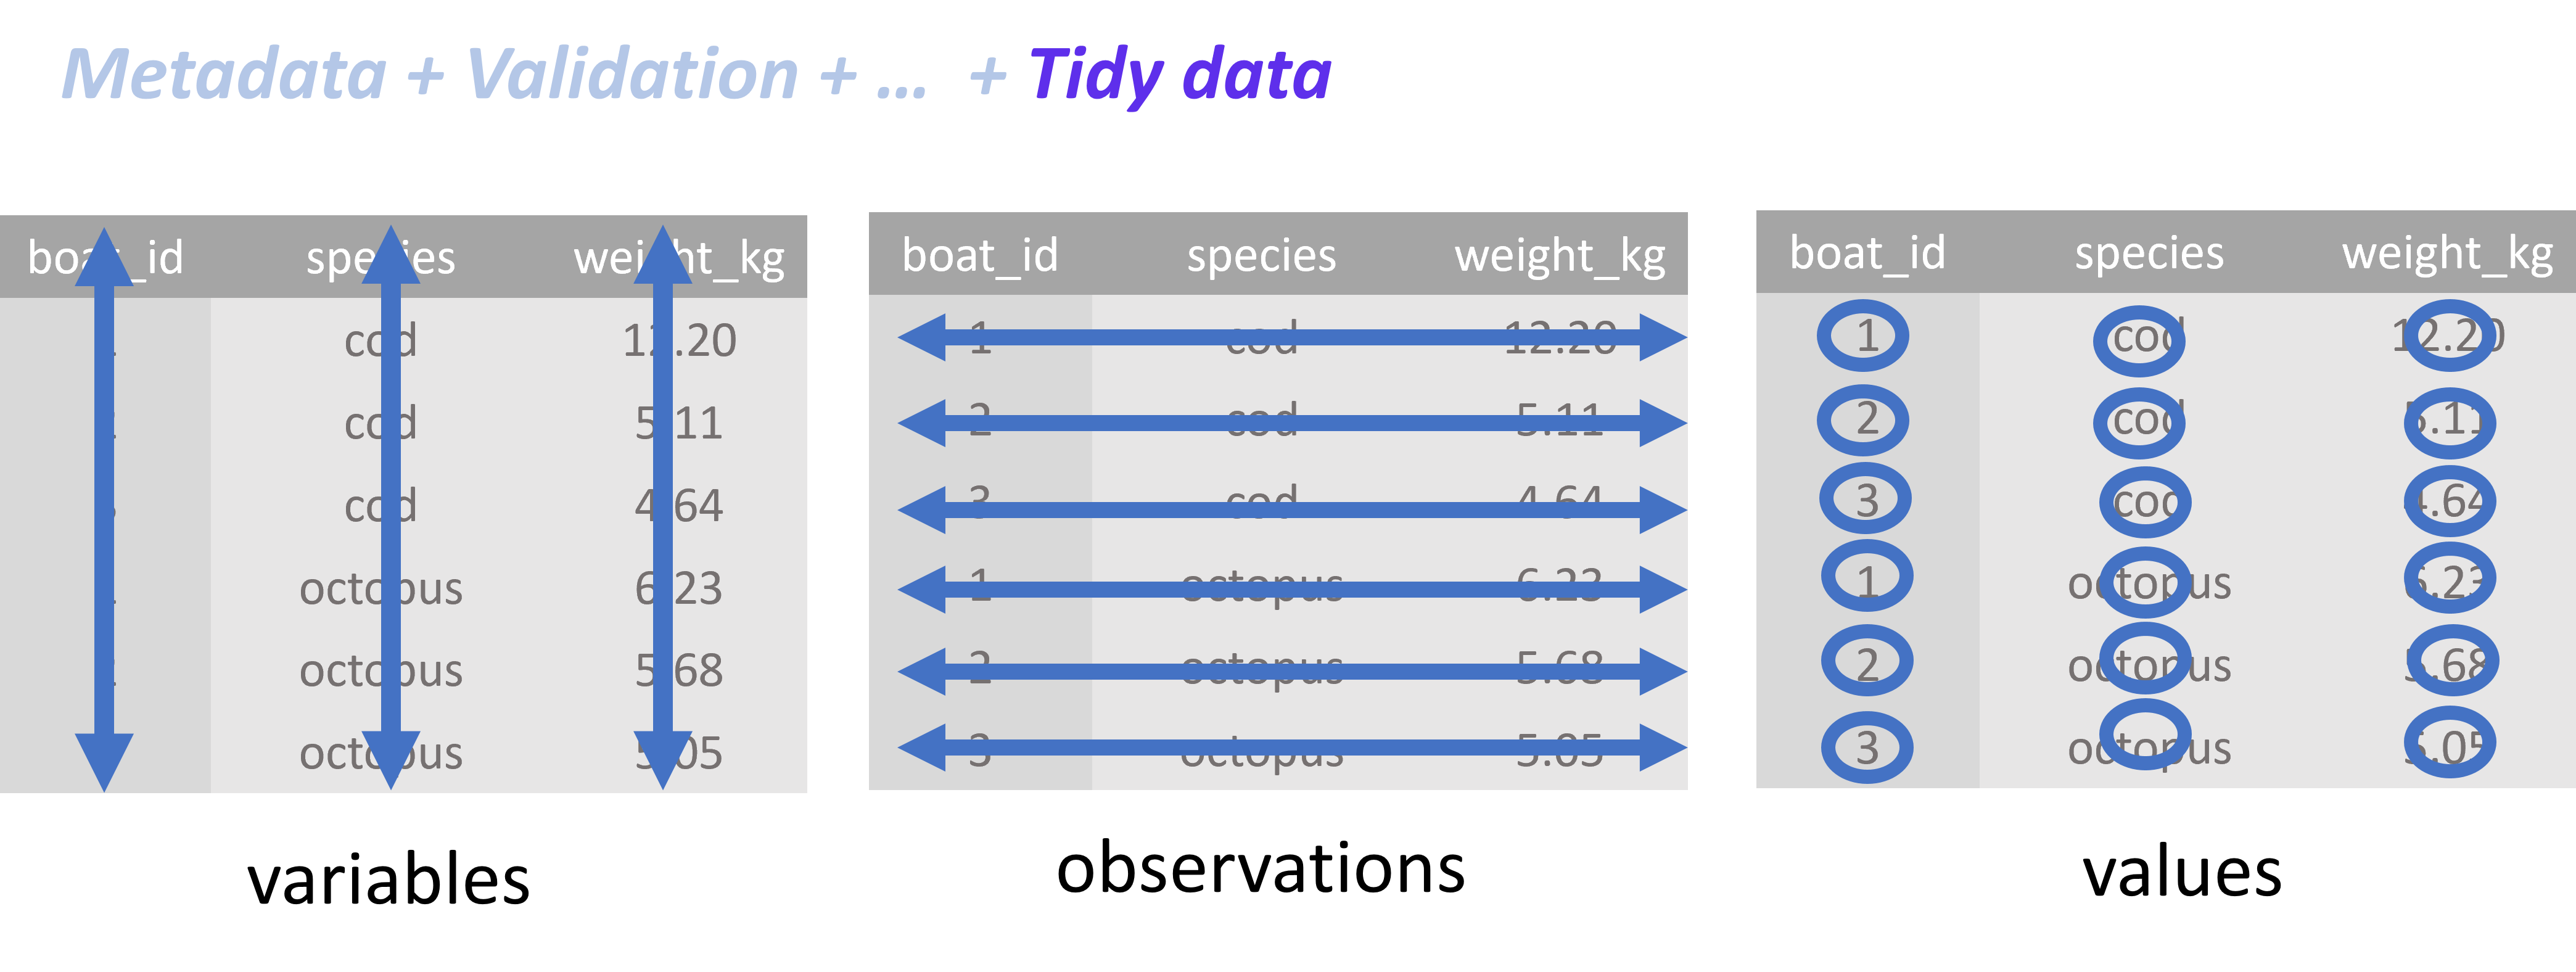
\includegraphics{tidydatavov.png}

\begin{center}\rule{0.5\linewidth}{0.5pt}\end{center}

Let's see a very simple example to show how R prefers tidy data: we will
use the (base R) \texttt{summary} function.

\hypertarget{try-this}{%
\subsubsection{📝 Try this:}\label{try-this}}

\hypertarget{tidy-data-1}{%
\paragraph{Tidy data}\label{tidy-data-1}}

See the first 10 rows of the penguins dataset. In the case of Palmer
penguins, a variable refers to an attribute of all the penguins, and an
observation refers to all the attributes of a single penguin.

\begin{Shaded}
\begin{Highlighting}[]
\NormalTok{penguins }\SpecialCharTok{\%\textgreater{}\%} \FunctionTok{head}\NormalTok{(}\DecValTok{10}\NormalTok{)}
\end{Highlighting}
\end{Shaded}

\begin{verbatim}
## # A tibble: 10 x 8
##    species island    bill_length_mm bill_depth_mm flipper_length_mm body_mass_g
##    <fct>   <fct>              <dbl>         <dbl>             <int>       <int>
##  1 Adelie  Torgersen           39.1          18.7               181        3750
##  2 Adelie  Torgersen           39.5          17.4               186        3800
##  3 Adelie  Torgersen           40.3          18                 195        3250
##  4 Adelie  Torgersen           NA            NA                  NA          NA
##  5 Adelie  Torgersen           36.7          19.3               193        3450
##  6 Adelie  Torgersen           39.3          20.6               190        3650
##  7 Adelie  Torgersen           38.9          17.8               181        3625
##  8 Adelie  Torgersen           39.2          19.6               195        4675
##  9 Adelie  Torgersen           34.1          18.1               193        3475
## 10 Adelie  Torgersen           42            20.2               190        4250
## # i 2 more variables: sex <fct>, year <int>
\end{verbatim}

Use the built-in function summary() to quickly summarise the data

\begin{Shaded}
\begin{Highlighting}[]
\FunctionTok{summary}\NormalTok{(penguins) }
\end{Highlighting}
\end{Shaded}

\begin{verbatim}
##       species          island    bill_length_mm  bill_depth_mm  
##  Adelie   :152   Biscoe   :168   Min.   :32.10   Min.   :13.10  
##  Chinstrap: 68   Dream    :124   1st Qu.:39.23   1st Qu.:15.60  
##  Gentoo   :124   Torgersen: 52   Median :44.45   Median :17.30  
##                                  Mean   :43.92   Mean   :17.15  
##                                  3rd Qu.:48.50   3rd Qu.:18.70  
##                                  Max.   :59.60   Max.   :21.50  
##                                  NA's   :2       NA's   :2      
##  flipper_length_mm  body_mass_g       sex           year     
##  Min.   :172.0     Min.   :2700   female:165   Min.   :2007  
##  1st Qu.:190.0     1st Qu.:3550   male  :168   1st Qu.:2007  
##  Median :197.0     Median :4050   NA's  : 11   Median :2008  
##  Mean   :200.9     Mean   :4202                Mean   :2008  
##  3rd Qu.:213.0     3rd Qu.:4750                3rd Qu.:2009  
##  Max.   :231.0     Max.   :6300                Max.   :2009  
##  NA's   :2         NA's   :2
\end{verbatim}

\hypertarget{untidy-data}{%
\paragraph{Untidy data}\label{untidy-data}}

Transform columns into rows and visualise data in R studio: does it look
bad? (Turning into messy from tidy)

\begin{Shaded}
\begin{Highlighting}[]
\NormalTok{(penguins }\SpecialCharTok{\%\textgreater{}\%} \FunctionTok{t}\NormalTok{()) }\SpecialCharTok{\%\textgreater{}\%} \FunctionTok{View}\NormalTok{()}
\end{Highlighting}
\end{Shaded}

How about this?

\begin{Shaded}
\begin{Highlighting}[]
\FunctionTok{summary}\NormalTok{(penguins}\SpecialCharTok{\%\textgreater{}\%}\FunctionTok{t}\NormalTok{())}
\end{Highlighting}
\end{Shaded}

\begin{verbatim}
##       V1                 V2                 V3                 V4           
##  Length:8           Length:8           Length:8           Length:8          
##  Class :character   Class :character   Class :character   Class :character  
##  Mode  :character   Mode  :character   Mode  :character   Mode  :character  
##       V5                 V6                 V7                 V8           
##  Length:8           Length:8           Length:8           Length:8          
##  Class :character   Class :character   Class :character   Class :character  
##  Mode  :character   Mode  :character   Mode  :character   Mode  :character  
##       V9                V10                V11                V12           
##  Length:8           Length:8           Length:8           Length:8          
##  Class :character   Class :character   Class :character   Class :character  
##  Mode  :character   Mode  :character   Mode  :character   Mode  :character  
##      V13                V14                V15                V16           
##  Length:8           Length:8           Length:8           Length:8          
##  Class :character   Class :character   Class :character   Class :character  
##  Mode  :character   Mode  :character   Mode  :character   Mode  :character  
##      V17                V18                V19                V20           
##  Length:8           Length:8           Length:8           Length:8          
##  Class :character   Class :character   Class :character   Class :character  
##  Mode  :character   Mode  :character   Mode  :character   Mode  :character  
##      V21                V22                V23                V24           
##  Length:8           Length:8           Length:8           Length:8          
##  Class :character   Class :character   Class :character   Class :character  
##  Mode  :character   Mode  :character   Mode  :character   Mode  :character  
##      V25                V26                V27                V28           
##  Length:8           Length:8           Length:8           Length:8          
##  Class :character   Class :character   Class :character   Class :character  
##  Mode  :character   Mode  :character   Mode  :character   Mode  :character  
##      V29                V30                V31                V32           
##  Length:8           Length:8           Length:8           Length:8          
##  Class :character   Class :character   Class :character   Class :character  
##  Mode  :character   Mode  :character   Mode  :character   Mode  :character  
##      V33                V34                V35                V36           
##  Length:8           Length:8           Length:8           Length:8          
##  Class :character   Class :character   Class :character   Class :character  
##  Mode  :character   Mode  :character   Mode  :character   Mode  :character  
##      V37                V38                V39                V40           
##  Length:8           Length:8           Length:8           Length:8          
##  Class :character   Class :character   Class :character   Class :character  
##  Mode  :character   Mode  :character   Mode  :character   Mode  :character  
##      V41                V42                V43                V44           
##  Length:8           Length:8           Length:8           Length:8          
##  Class :character   Class :character   Class :character   Class :character  
##  Mode  :character   Mode  :character   Mode  :character   Mode  :character  
##      V45                V46                V47                V48           
##  Length:8           Length:8           Length:8           Length:8          
##  Class :character   Class :character   Class :character   Class :character  
##  Mode  :character   Mode  :character   Mode  :character   Mode  :character  
##      V49                V50                V51                V52           
##  Length:8           Length:8           Length:8           Length:8          
##  Class :character   Class :character   Class :character   Class :character  
##  Mode  :character   Mode  :character   Mode  :character   Mode  :character  
##      V53                V54                V55                V56           
##  Length:8           Length:8           Length:8           Length:8          
##  Class :character   Class :character   Class :character   Class :character  
##  Mode  :character   Mode  :character   Mode  :character   Mode  :character  
##      V57                V58                V59                V60           
##  Length:8           Length:8           Length:8           Length:8          
##  Class :character   Class :character   Class :character   Class :character  
##  Mode  :character   Mode  :character   Mode  :character   Mode  :character  
##      V61                V62                V63                V64           
##  Length:8           Length:8           Length:8           Length:8          
##  Class :character   Class :character   Class :character   Class :character  
##  Mode  :character   Mode  :character   Mode  :character   Mode  :character  
##      V65                V66                V67                V68           
##  Length:8           Length:8           Length:8           Length:8          
##  Class :character   Class :character   Class :character   Class :character  
##  Mode  :character   Mode  :character   Mode  :character   Mode  :character  
##      V69                V70                V71                V72           
##  Length:8           Length:8           Length:8           Length:8          
##  Class :character   Class :character   Class :character   Class :character  
##  Mode  :character   Mode  :character   Mode  :character   Mode  :character  
##      V73                V74                V75                V76           
##  Length:8           Length:8           Length:8           Length:8          
##  Class :character   Class :character   Class :character   Class :character  
##  Mode  :character   Mode  :character   Mode  :character   Mode  :character  
##      V77                V78                V79                V80           
##  Length:8           Length:8           Length:8           Length:8          
##  Class :character   Class :character   Class :character   Class :character  
##  Mode  :character   Mode  :character   Mode  :character   Mode  :character  
##      V81                V82                V83                V84           
##  Length:8           Length:8           Length:8           Length:8          
##  Class :character   Class :character   Class :character   Class :character  
##  Mode  :character   Mode  :character   Mode  :character   Mode  :character  
##      V85                V86                V87                V88           
##  Length:8           Length:8           Length:8           Length:8          
##  Class :character   Class :character   Class :character   Class :character  
##  Mode  :character   Mode  :character   Mode  :character   Mode  :character  
##      V89                V90                V91                V92           
##  Length:8           Length:8           Length:8           Length:8          
##  Class :character   Class :character   Class :character   Class :character  
##  Mode  :character   Mode  :character   Mode  :character   Mode  :character  
##      V93                V94                V95                V96           
##  Length:8           Length:8           Length:8           Length:8          
##  Class :character   Class :character   Class :character   Class :character  
##  Mode  :character   Mode  :character   Mode  :character   Mode  :character  
##      V97                V98                V99                V100          
##  Length:8           Length:8           Length:8           Length:8          
##  Class :character   Class :character   Class :character   Class :character  
##  Mode  :character   Mode  :character   Mode  :character   Mode  :character  
##      V101               V102               V103               V104          
##  Length:8           Length:8           Length:8           Length:8          
##  Class :character   Class :character   Class :character   Class :character  
##  Mode  :character   Mode  :character   Mode  :character   Mode  :character  
##      V105               V106               V107               V108          
##  Length:8           Length:8           Length:8           Length:8          
##  Class :character   Class :character   Class :character   Class :character  
##  Mode  :character   Mode  :character   Mode  :character   Mode  :character  
##      V109               V110               V111               V112          
##  Length:8           Length:8           Length:8           Length:8          
##  Class :character   Class :character   Class :character   Class :character  
##  Mode  :character   Mode  :character   Mode  :character   Mode  :character  
##      V113               V114               V115               V116          
##  Length:8           Length:8           Length:8           Length:8          
##  Class :character   Class :character   Class :character   Class :character  
##  Mode  :character   Mode  :character   Mode  :character   Mode  :character  
##      V117               V118               V119               V120          
##  Length:8           Length:8           Length:8           Length:8          
##  Class :character   Class :character   Class :character   Class :character  
##  Mode  :character   Mode  :character   Mode  :character   Mode  :character  
##      V121               V122               V123               V124          
##  Length:8           Length:8           Length:8           Length:8          
##  Class :character   Class :character   Class :character   Class :character  
##  Mode  :character   Mode  :character   Mode  :character   Mode  :character  
##      V125               V126               V127               V128          
##  Length:8           Length:8           Length:8           Length:8          
##  Class :character   Class :character   Class :character   Class :character  
##  Mode  :character   Mode  :character   Mode  :character   Mode  :character  
##      V129               V130               V131               V132          
##  Length:8           Length:8           Length:8           Length:8          
##  Class :character   Class :character   Class :character   Class :character  
##  Mode  :character   Mode  :character   Mode  :character   Mode  :character  
##      V133               V134               V135               V136          
##  Length:8           Length:8           Length:8           Length:8          
##  Class :character   Class :character   Class :character   Class :character  
##  Mode  :character   Mode  :character   Mode  :character   Mode  :character  
##      V137               V138               V139               V140          
##  Length:8           Length:8           Length:8           Length:8          
##  Class :character   Class :character   Class :character   Class :character  
##  Mode  :character   Mode  :character   Mode  :character   Mode  :character  
##      V141               V142               V143               V144          
##  Length:8           Length:8           Length:8           Length:8          
##  Class :character   Class :character   Class :character   Class :character  
##  Mode  :character   Mode  :character   Mode  :character   Mode  :character  
##      V145               V146               V147               V148          
##  Length:8           Length:8           Length:8           Length:8          
##  Class :character   Class :character   Class :character   Class :character  
##  Mode  :character   Mode  :character   Mode  :character   Mode  :character  
##      V149               V150               V151               V152          
##  Length:8           Length:8           Length:8           Length:8          
##  Class :character   Class :character   Class :character   Class :character  
##  Mode  :character   Mode  :character   Mode  :character   Mode  :character  
##      V153               V154               V155               V156          
##  Length:8           Length:8           Length:8           Length:8          
##  Class :character   Class :character   Class :character   Class :character  
##  Mode  :character   Mode  :character   Mode  :character   Mode  :character  
##      V157               V158               V159               V160          
##  Length:8           Length:8           Length:8           Length:8          
##  Class :character   Class :character   Class :character   Class :character  
##  Mode  :character   Mode  :character   Mode  :character   Mode  :character  
##      V161               V162               V163               V164          
##  Length:8           Length:8           Length:8           Length:8          
##  Class :character   Class :character   Class :character   Class :character  
##  Mode  :character   Mode  :character   Mode  :character   Mode  :character  
##      V165               V166               V167               V168          
##  Length:8           Length:8           Length:8           Length:8          
##  Class :character   Class :character   Class :character   Class :character  
##  Mode  :character   Mode  :character   Mode  :character   Mode  :character  
##      V169               V170               V171               V172          
##  Length:8           Length:8           Length:8           Length:8          
##  Class :character   Class :character   Class :character   Class :character  
##  Mode  :character   Mode  :character   Mode  :character   Mode  :character  
##      V173               V174               V175               V176          
##  Length:8           Length:8           Length:8           Length:8          
##  Class :character   Class :character   Class :character   Class :character  
##  Mode  :character   Mode  :character   Mode  :character   Mode  :character  
##      V177               V178               V179               V180          
##  Length:8           Length:8           Length:8           Length:8          
##  Class :character   Class :character   Class :character   Class :character  
##  Mode  :character   Mode  :character   Mode  :character   Mode  :character  
##      V181               V182               V183               V184          
##  Length:8           Length:8           Length:8           Length:8          
##  Class :character   Class :character   Class :character   Class :character  
##  Mode  :character   Mode  :character   Mode  :character   Mode  :character  
##      V185               V186               V187               V188          
##  Length:8           Length:8           Length:8           Length:8          
##  Class :character   Class :character   Class :character   Class :character  
##  Mode  :character   Mode  :character   Mode  :character   Mode  :character  
##      V189               V190               V191               V192          
##  Length:8           Length:8           Length:8           Length:8          
##  Class :character   Class :character   Class :character   Class :character  
##  Mode  :character   Mode  :character   Mode  :character   Mode  :character  
##      V193               V194               V195               V196          
##  Length:8           Length:8           Length:8           Length:8          
##  Class :character   Class :character   Class :character   Class :character  
##  Mode  :character   Mode  :character   Mode  :character   Mode  :character  
##      V197               V198               V199               V200          
##  Length:8           Length:8           Length:8           Length:8          
##  Class :character   Class :character   Class :character   Class :character  
##  Mode  :character   Mode  :character   Mode  :character   Mode  :character  
##      V201               V202               V203               V204          
##  Length:8           Length:8           Length:8           Length:8          
##  Class :character   Class :character   Class :character   Class :character  
##  Mode  :character   Mode  :character   Mode  :character   Mode  :character  
##      V205               V206               V207               V208          
##  Length:8           Length:8           Length:8           Length:8          
##  Class :character   Class :character   Class :character   Class :character  
##  Mode  :character   Mode  :character   Mode  :character   Mode  :character  
##      V209               V210               V211               V212          
##  Length:8           Length:8           Length:8           Length:8          
##  Class :character   Class :character   Class :character   Class :character  
##  Mode  :character   Mode  :character   Mode  :character   Mode  :character  
##      V213               V214               V215               V216          
##  Length:8           Length:8           Length:8           Length:8          
##  Class :character   Class :character   Class :character   Class :character  
##  Mode  :character   Mode  :character   Mode  :character   Mode  :character  
##      V217               V218               V219               V220          
##  Length:8           Length:8           Length:8           Length:8          
##  Class :character   Class :character   Class :character   Class :character  
##  Mode  :character   Mode  :character   Mode  :character   Mode  :character  
##      V221               V222               V223               V224          
##  Length:8           Length:8           Length:8           Length:8          
##  Class :character   Class :character   Class :character   Class :character  
##  Mode  :character   Mode  :character   Mode  :character   Mode  :character  
##      V225               V226               V227               V228          
##  Length:8           Length:8           Length:8           Length:8          
##  Class :character   Class :character   Class :character   Class :character  
##  Mode  :character   Mode  :character   Mode  :character   Mode  :character  
##      V229               V230               V231               V232          
##  Length:8           Length:8           Length:8           Length:8          
##  Class :character   Class :character   Class :character   Class :character  
##  Mode  :character   Mode  :character   Mode  :character   Mode  :character  
##      V233               V234               V235               V236          
##  Length:8           Length:8           Length:8           Length:8          
##  Class :character   Class :character   Class :character   Class :character  
##  Mode  :character   Mode  :character   Mode  :character   Mode  :character  
##      V237               V238               V239               V240          
##  Length:8           Length:8           Length:8           Length:8          
##  Class :character   Class :character   Class :character   Class :character  
##  Mode  :character   Mode  :character   Mode  :character   Mode  :character  
##      V241               V242               V243               V244          
##  Length:8           Length:8           Length:8           Length:8          
##  Class :character   Class :character   Class :character   Class :character  
##  Mode  :character   Mode  :character   Mode  :character   Mode  :character  
##      V245               V246               V247               V248          
##  Length:8           Length:8           Length:8           Length:8          
##  Class :character   Class :character   Class :character   Class :character  
##  Mode  :character   Mode  :character   Mode  :character   Mode  :character  
##      V249               V250               V251               V252          
##  Length:8           Length:8           Length:8           Length:8          
##  Class :character   Class :character   Class :character   Class :character  
##  Mode  :character   Mode  :character   Mode  :character   Mode  :character  
##      V253               V254               V255               V256          
##  Length:8           Length:8           Length:8           Length:8          
##  Class :character   Class :character   Class :character   Class :character  
##  Mode  :character   Mode  :character   Mode  :character   Mode  :character  
##      V257               V258               V259               V260          
##  Length:8           Length:8           Length:8           Length:8          
##  Class :character   Class :character   Class :character   Class :character  
##  Mode  :character   Mode  :character   Mode  :character   Mode  :character  
##      V261               V262               V263               V264          
##  Length:8           Length:8           Length:8           Length:8          
##  Class :character   Class :character   Class :character   Class :character  
##  Mode  :character   Mode  :character   Mode  :character   Mode  :character  
##      V265               V266               V267               V268          
##  Length:8           Length:8           Length:8           Length:8          
##  Class :character   Class :character   Class :character   Class :character  
##  Mode  :character   Mode  :character   Mode  :character   Mode  :character  
##      V269               V270               V271               V272          
##  Length:8           Length:8           Length:8           Length:8          
##  Class :character   Class :character   Class :character   Class :character  
##  Mode  :character   Mode  :character   Mode  :character   Mode  :character  
##      V273               V274               V275               V276          
##  Length:8           Length:8           Length:8           Length:8          
##  Class :character   Class :character   Class :character   Class :character  
##  Mode  :character   Mode  :character   Mode  :character   Mode  :character  
##      V277               V278               V279               V280          
##  Length:8           Length:8           Length:8           Length:8          
##  Class :character   Class :character   Class :character   Class :character  
##  Mode  :character   Mode  :character   Mode  :character   Mode  :character  
##      V281               V282               V283               V284          
##  Length:8           Length:8           Length:8           Length:8          
##  Class :character   Class :character   Class :character   Class :character  
##  Mode  :character   Mode  :character   Mode  :character   Mode  :character  
##      V285               V286               V287               V288          
##  Length:8           Length:8           Length:8           Length:8          
##  Class :character   Class :character   Class :character   Class :character  
##  Mode  :character   Mode  :character   Mode  :character   Mode  :character  
##      V289               V290               V291               V292          
##  Length:8           Length:8           Length:8           Length:8          
##  Class :character   Class :character   Class :character   Class :character  
##  Mode  :character   Mode  :character   Mode  :character   Mode  :character  
##      V293               V294               V295               V296          
##  Length:8           Length:8           Length:8           Length:8          
##  Class :character   Class :character   Class :character   Class :character  
##  Mode  :character   Mode  :character   Mode  :character   Mode  :character  
##      V297               V298               V299               V300          
##  Length:8           Length:8           Length:8           Length:8          
##  Class :character   Class :character   Class :character   Class :character  
##  Mode  :character   Mode  :character   Mode  :character   Mode  :character  
##      V301               V302               V303               V304          
##  Length:8           Length:8           Length:8           Length:8          
##  Class :character   Class :character   Class :character   Class :character  
##  Mode  :character   Mode  :character   Mode  :character   Mode  :character  
##      V305               V306               V307               V308          
##  Length:8           Length:8           Length:8           Length:8          
##  Class :character   Class :character   Class :character   Class :character  
##  Mode  :character   Mode  :character   Mode  :character   Mode  :character  
##      V309               V310               V311               V312          
##  Length:8           Length:8           Length:8           Length:8          
##  Class :character   Class :character   Class :character   Class :character  
##  Mode  :character   Mode  :character   Mode  :character   Mode  :character  
##      V313               V314               V315               V316          
##  Length:8           Length:8           Length:8           Length:8          
##  Class :character   Class :character   Class :character   Class :character  
##  Mode  :character   Mode  :character   Mode  :character   Mode  :character  
##      V317               V318               V319               V320          
##  Length:8           Length:8           Length:8           Length:8          
##  Class :character   Class :character   Class :character   Class :character  
##  Mode  :character   Mode  :character   Mode  :character   Mode  :character  
##      V321               V322               V323               V324          
##  Length:8           Length:8           Length:8           Length:8          
##  Class :character   Class :character   Class :character   Class :character  
##  Mode  :character   Mode  :character   Mode  :character   Mode  :character  
##      V325               V326               V327               V328          
##  Length:8           Length:8           Length:8           Length:8          
##  Class :character   Class :character   Class :character   Class :character  
##  Mode  :character   Mode  :character   Mode  :character   Mode  :character  
##      V329               V330               V331               V332          
##  Length:8           Length:8           Length:8           Length:8          
##  Class :character   Class :character   Class :character   Class :character  
##  Mode  :character   Mode  :character   Mode  :character   Mode  :character  
##      V333               V334               V335               V336          
##  Length:8           Length:8           Length:8           Length:8          
##  Class :character   Class :character   Class :character   Class :character  
##  Mode  :character   Mode  :character   Mode  :character   Mode  :character  
##      V337               V338               V339               V340          
##  Length:8           Length:8           Length:8           Length:8          
##  Class :character   Class :character   Class :character   Class :character  
##  Mode  :character   Mode  :character   Mode  :character   Mode  :character  
##      V341               V342               V343               V344          
##  Length:8           Length:8           Length:8           Length:8          
##  Class :character   Class :character   Class :character   Class :character  
##  Mode  :character   Mode  :character   Mode  :character   Mode  :character
\end{verbatim}

\begin{center}\rule{0.5\linewidth}{0.5pt}\end{center}

\hypertarget{tidying-data-with-tidyr}{%
\subsubsection{\texorpdfstring{\textbf{Tidying data with
tidyr}}{Tidying data with tidyr}}\label{tidying-data-with-tidyr}}

\texttt{tidyr} is one of the packages used to get data into a tidy
format.

• \textbf{pivot\_longer} -- convert to tidy

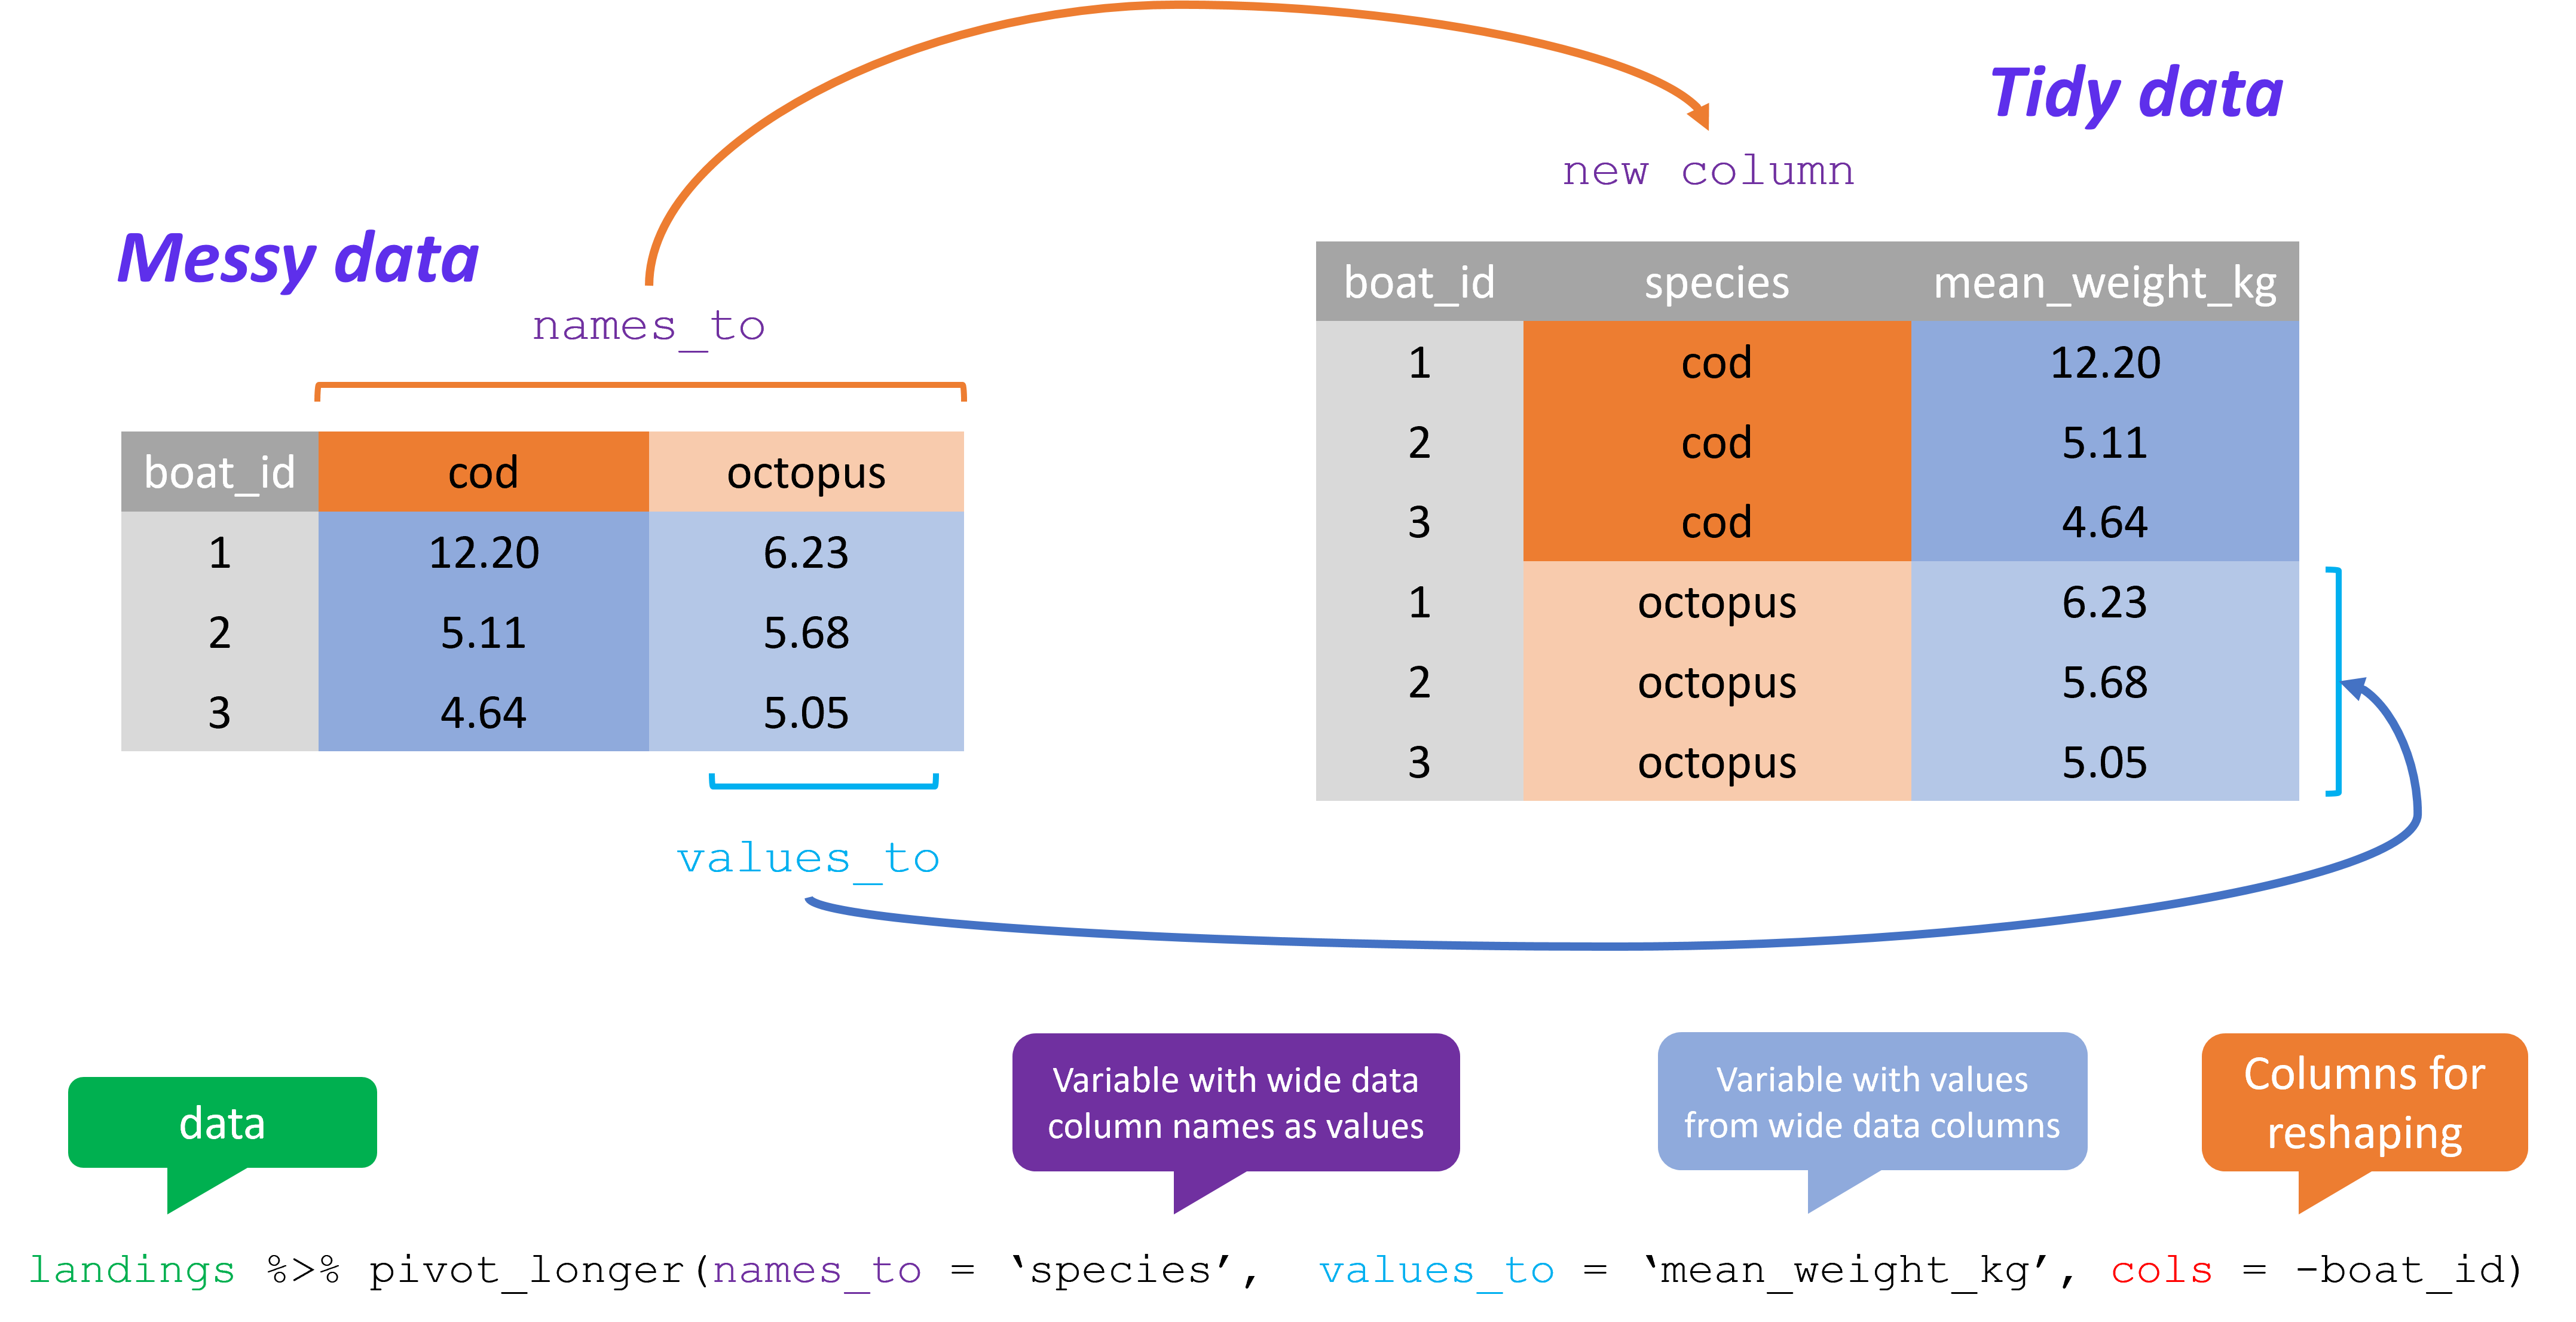
\includegraphics{pivot_longer.png}

• \textbf{pivot\_wider} -- convert to untidy (because there is nothing
intrinsically wrong with it!)

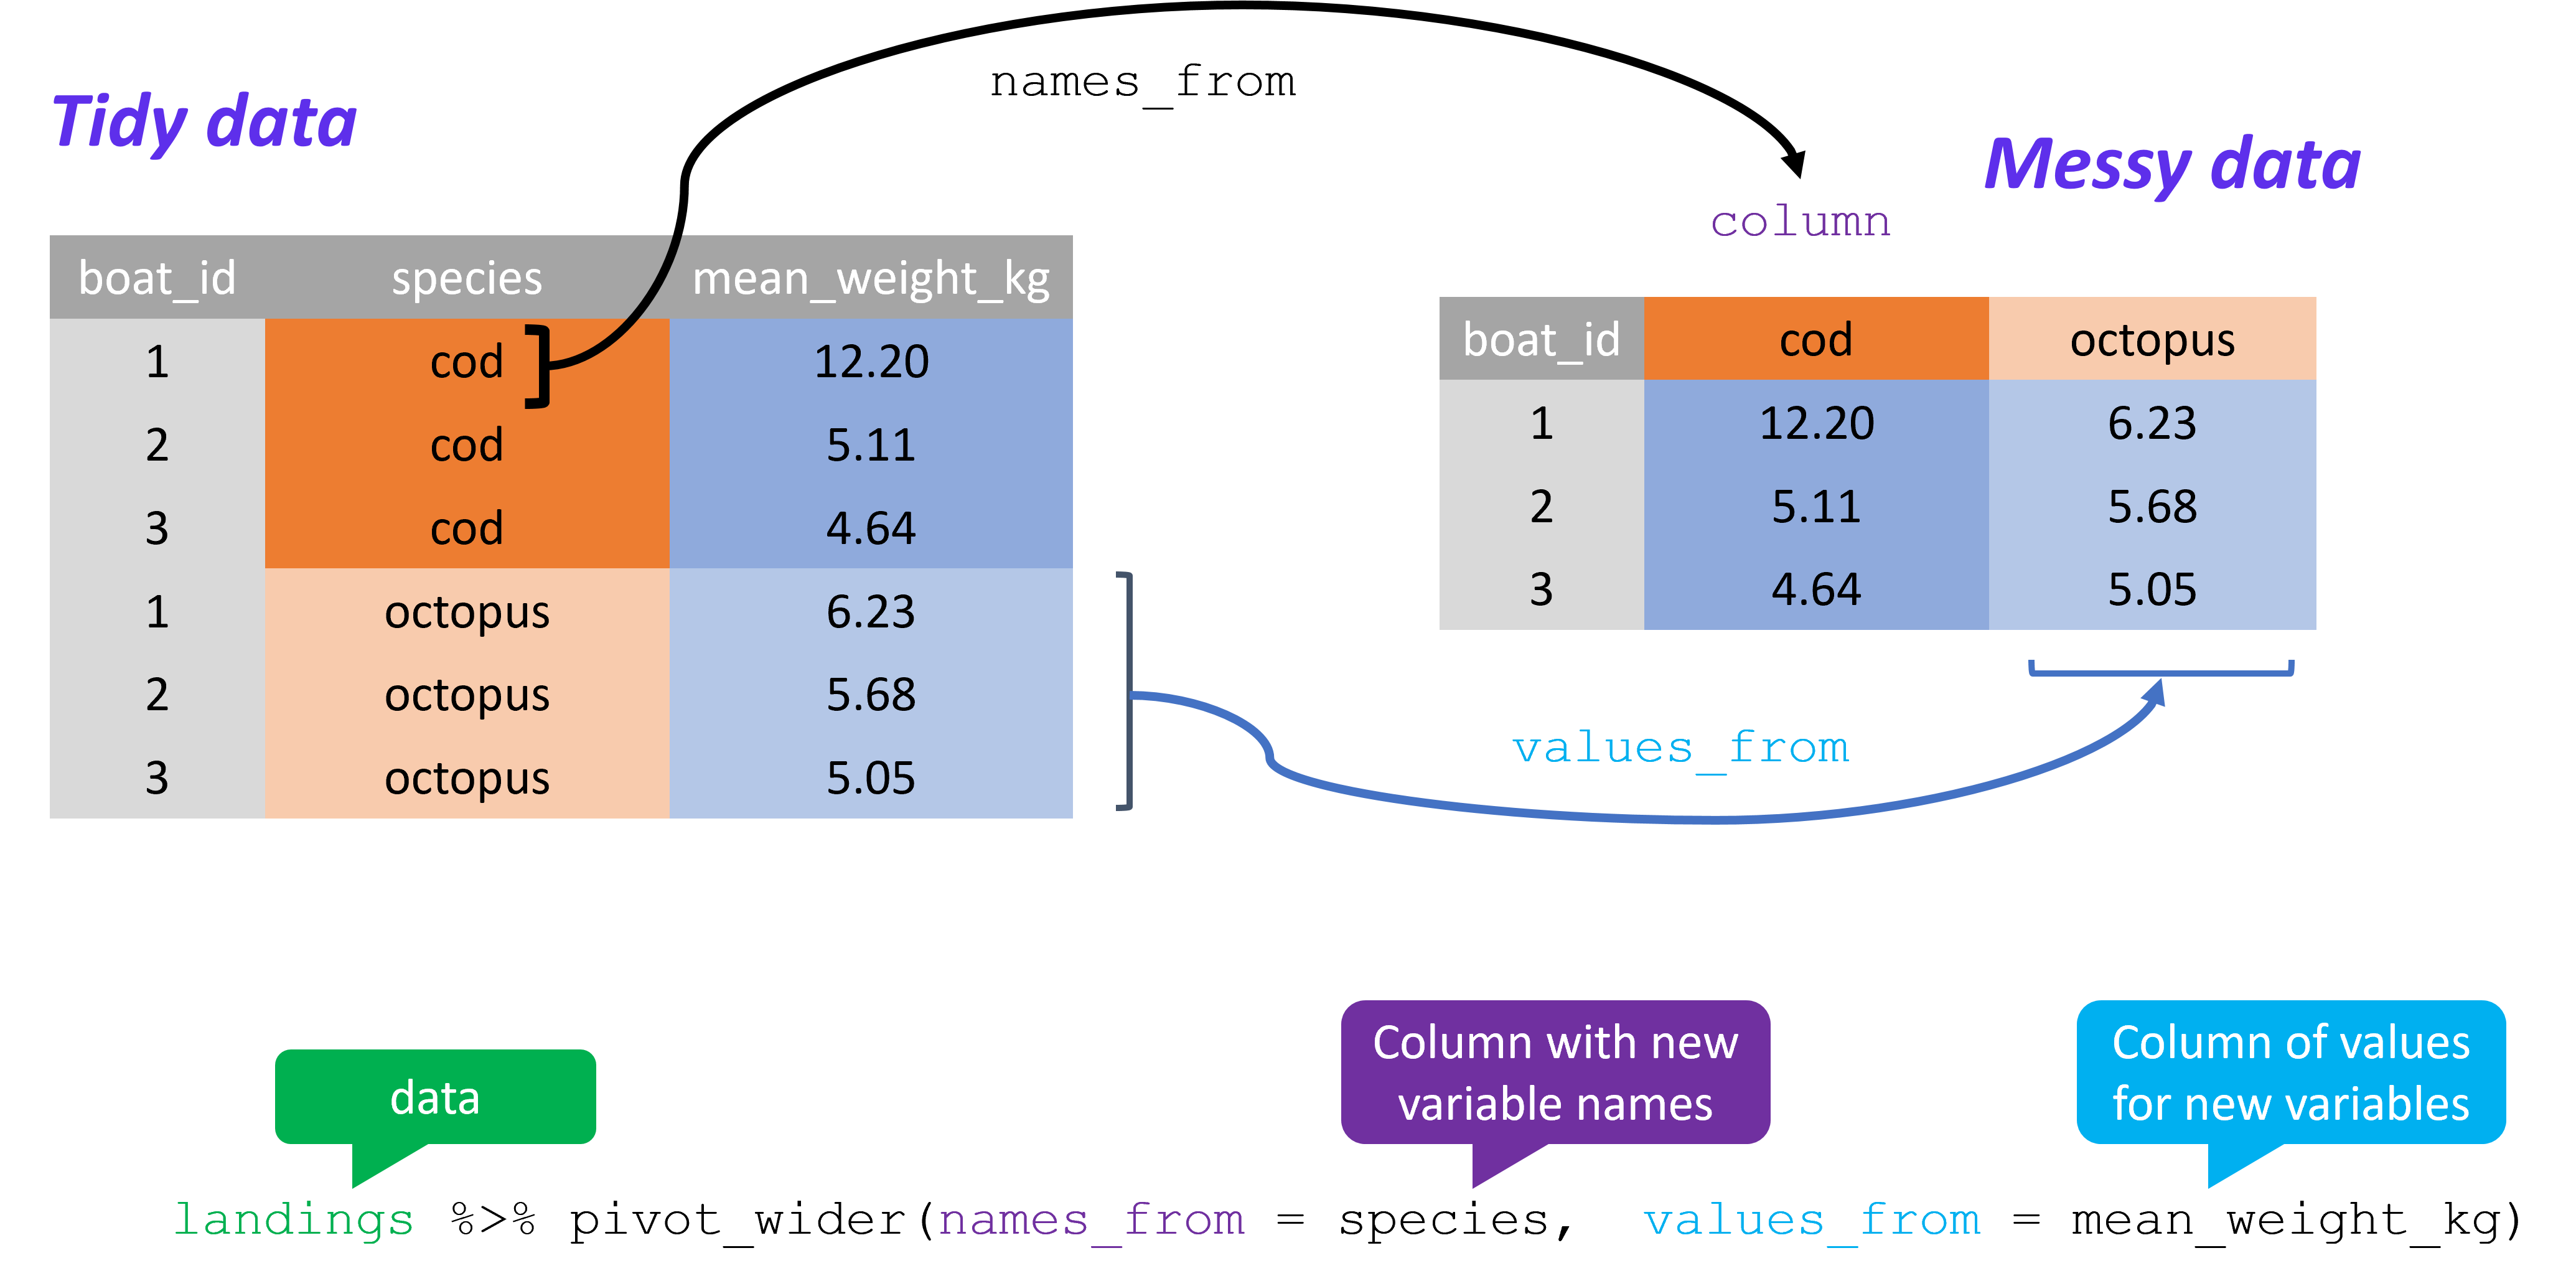
\includegraphics{pivot_wider.png}

\begin{center}\rule{0.5\linewidth}{0.5pt}\end{center}

\hypertarget{data-manipulation-with-dplyr}{%
\subsection{Data Manipulation with
dplyr}\label{data-manipulation-with-dplyr}}

Besides tidyr, dplyr is probably the most widely used tidyverse package.
It is used to manipulate and transform data. The 5 main dplyr verbs that
you will come across many times throughout this course:

\textbf{filter:} select a subset of rows/observations

\textbf{select:} choose which columns/variables to work with.

\textbf{arrange:} change order of rows, by default arranging happens in
ascending order

\textbf{mutate:} update or create new columns of a data frame.

\textbf{summarise:} turn many observations into a single data point (eg
mean, max)

\textbf{group\_by:} allows actions to be performed by group (group\_by
is often followed by summarise)

\href{https://teachingr.com/content/the-5-verbs-of-dplyr/the-5-verbs-of-dplyr-article.html\#:~:text=The\%20magic\%20of\%20dplyr\%20is\%20that\%20with\%20just,of\%20dplyr\%3A\%20select\%2C\%20filter\%2C\%20arrange\%2C\%20mutate\%2C\%20and\%20summarize.}{https://teachingr.com/content/the-5-verbs-of-dplyr}

\begin{center}\rule{0.5\linewidth}{0.5pt}\end{center}

\hypertarget{joining-datasets}{%
\subsubsection{Joining datasets}\label{joining-datasets}}

Another very useful dplyr capability that is essential in research, is
to help joining datasets.

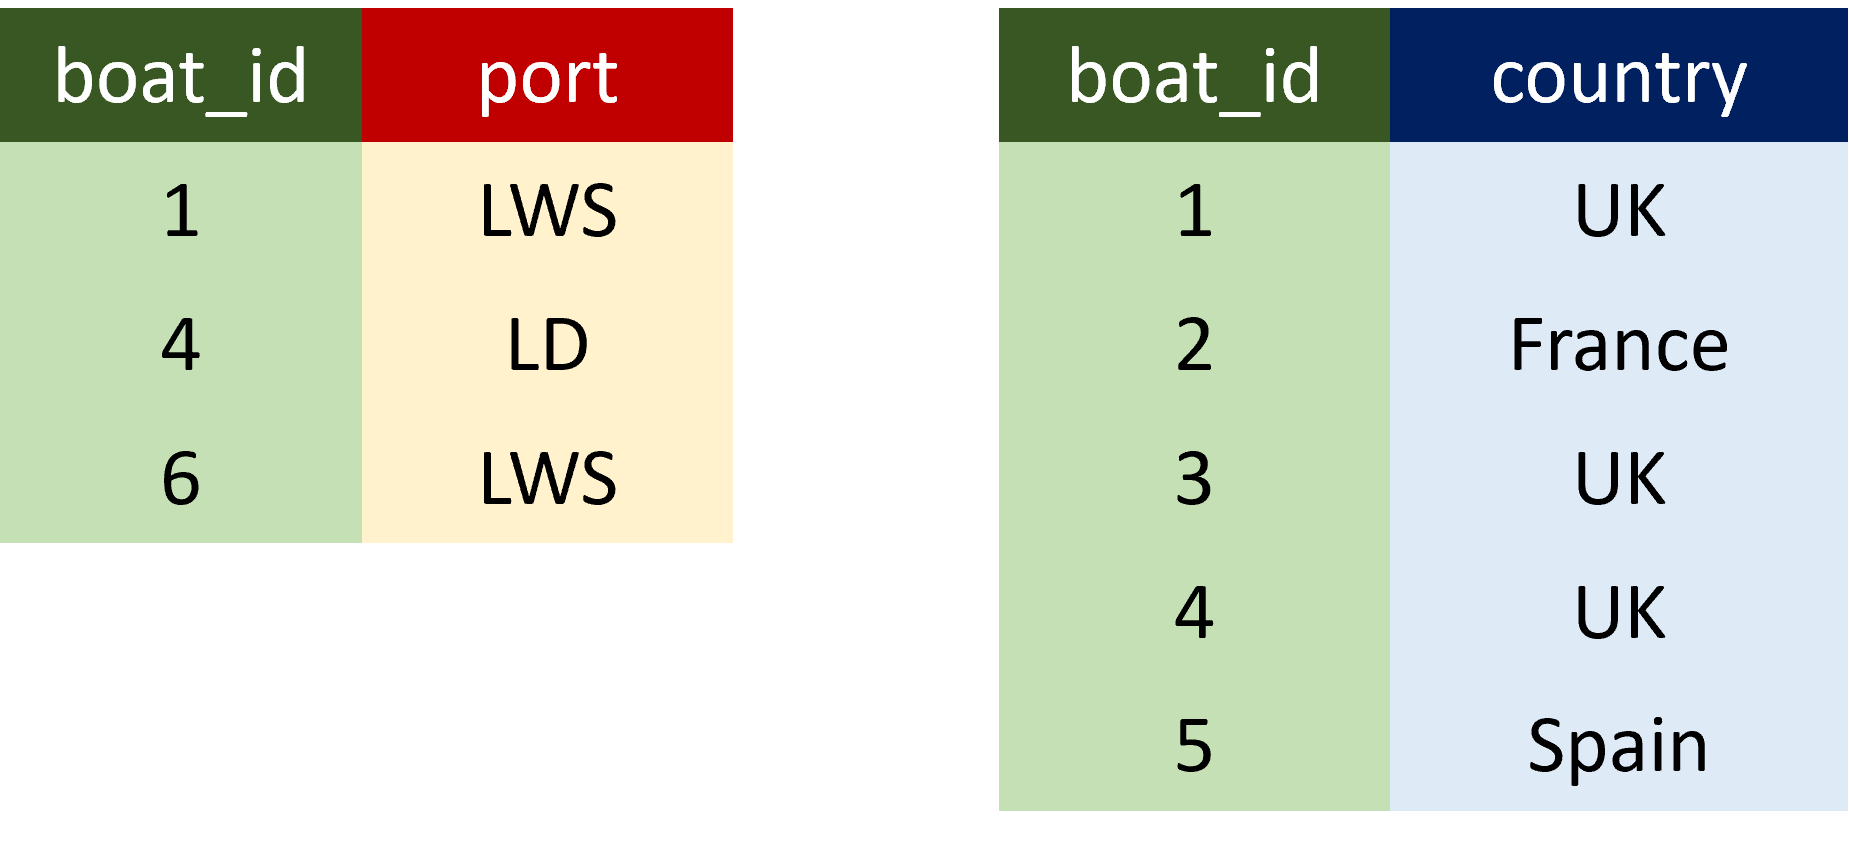
\includegraphics[width=3.42708in,height=\textheight]{initialdata.png}

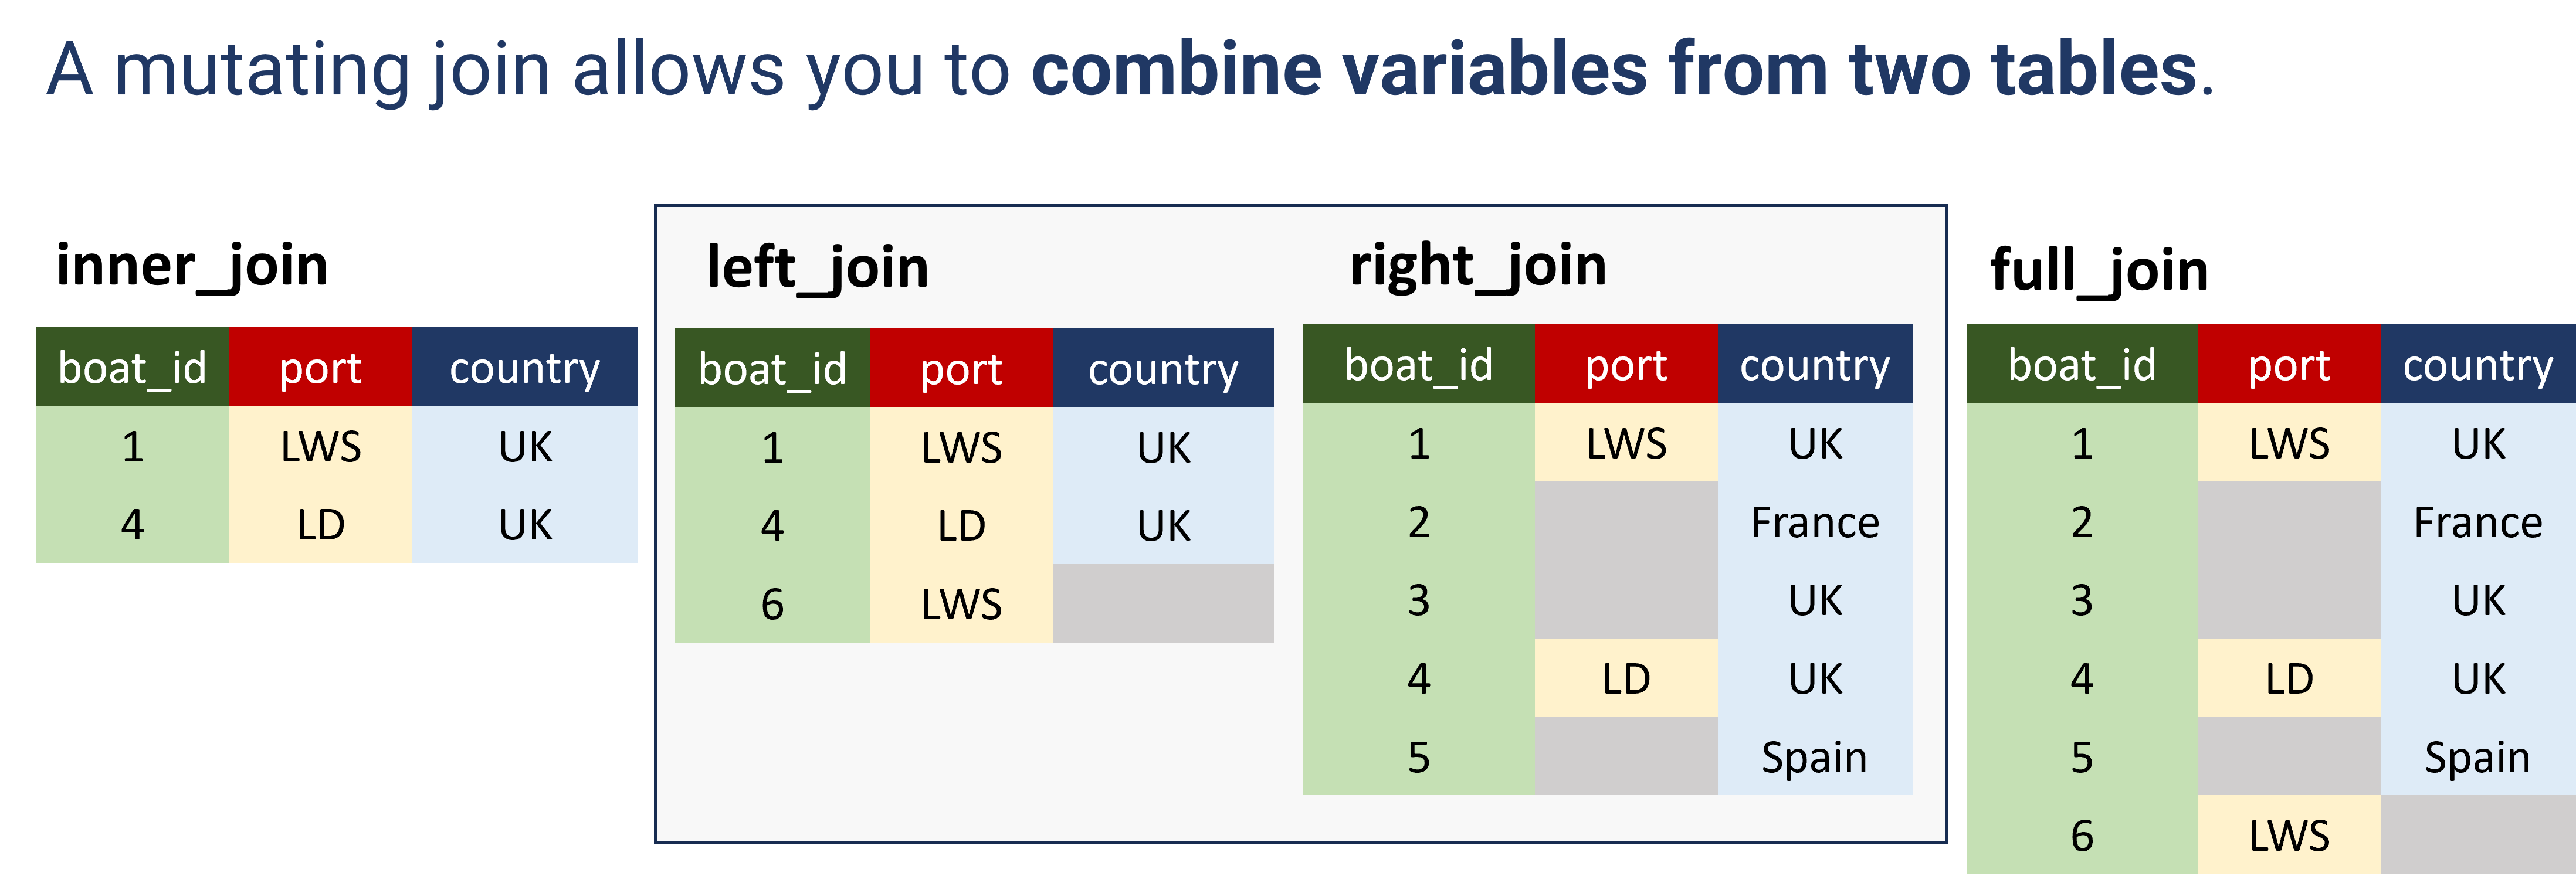
\includegraphics{mutatejoin.png}

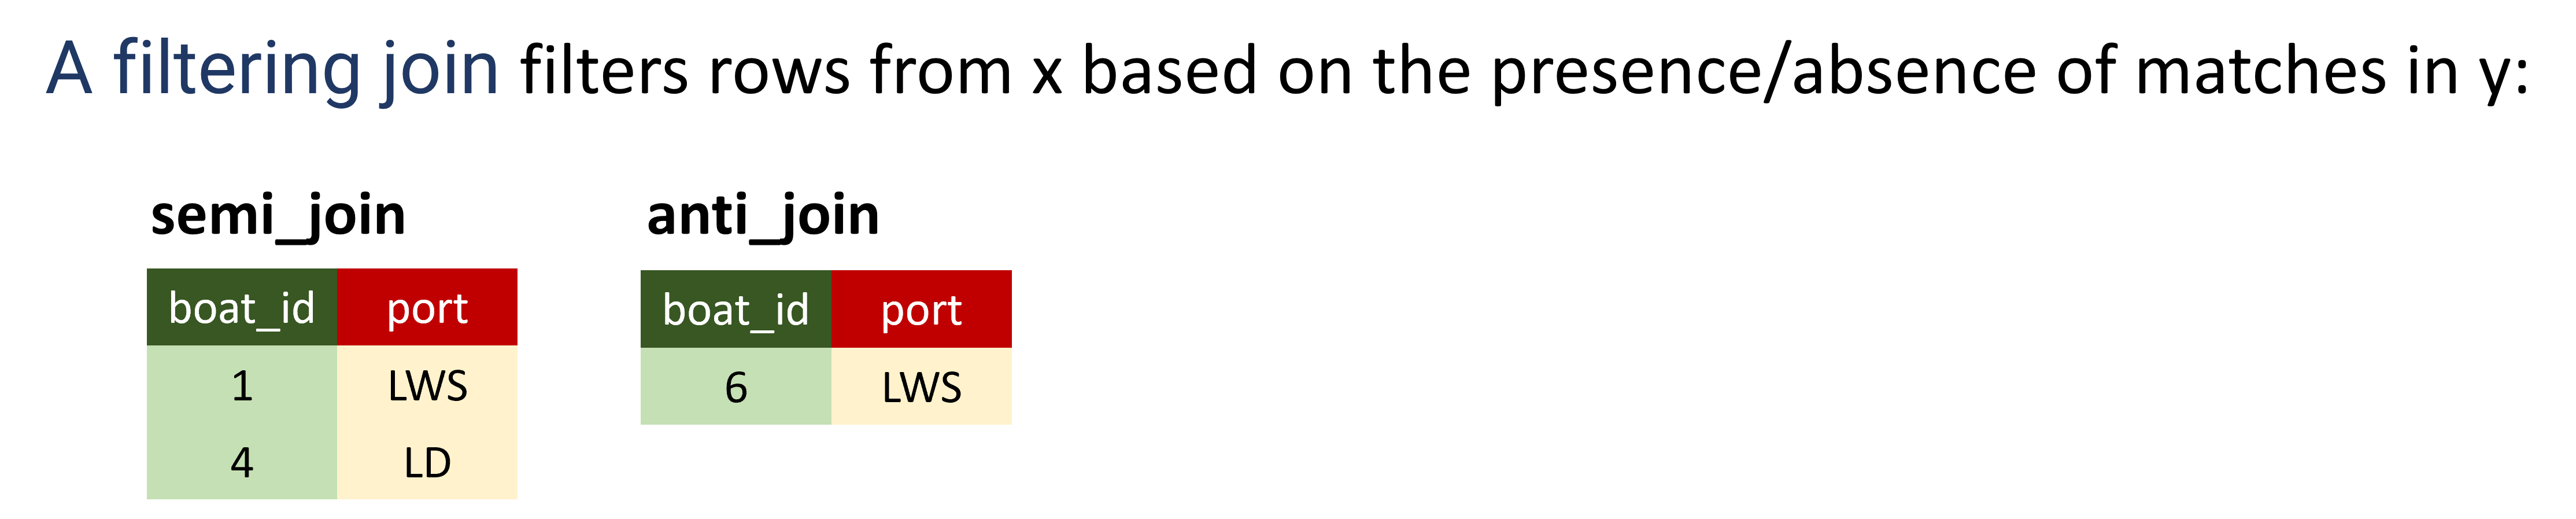
\includegraphics{filterjoin.png}

\hypertarget{there-is-also-fuzzyjoinfuzzy_join-allows-partial-and-inexact-matching}{%
\paragraph{\texorpdfstring{☝️ \textbf{There is also
\texttt{fuzzyjoin::fuzzy\_join}} (\#allows partial and inexact
matching)}{☝️ There is also fuzzyjoin::fuzzy\_join (\#allows partial and inexact matching)}}\label{there-is-also-fuzzyjoinfuzzy_join-allows-partial-and-inexact-matching}}

\hypertarget{to-summarise}{%
\subsubsection{\texorpdfstring{\textbf{To
summarise}:}{To summarise:}}\label{to-summarise}}

\begin{itemize}
\item
  using the tidyverse will help to organise and streamline your data
  analysis workflow in a consistent way
\item
  it is easy to learn and there is help available: there is a huge
  number of online resources and a very welcoming community organising
  events, meetups, coding clubs...

  Example:
  \href{https://github.com/rfordatascience/tidytuesday/tree/master}{rfordatascience/tidytuesday:
  Official repo for the \#tidytuesday project (github.com)}
\end{itemize}

In the following sessions, you will have the opportunity to use the
tidyverse and base R in practice

\hypertarget{to-finalise-some-more-resources}{%
\subsubsection{To finalise, some more
resources:}\label{to-finalise-some-more-resources}}

\textbf{Here you can see animations of the above:}

\url{https://tidydatatutor.com/index.html}

\url{https://www.garrickadenbuie.com/project/tidyexplain/\#pivot-wider-and-longer}

\textbf{Many cheat sheets:}
\href{https://posit.co/resources/cheatsheets/}{Cheatsheets - Posit}

\textbf{learn}

\url{https://www.tidyverse.org/learn/}

\url{https://r4ds.hadley.nz/}

\href{https://www.datacamp.com/cheat-sheet/tidyverse-cheat-sheet-for-beginners}{Tidyverse
Cheat Sheet For Beginners \textbar{} DataCamp}

\url{https://rstudio-education.github.io/tidyverse-cookbook/transform-tables.html}

\textbf{and practice}

\url{https://www.jvcasillas.com/untidydata/}

\end{document}
